% ABC2Vec Paper
% v1.0 - March 2026

\documentclass[]{interact}

\usepackage{epstopdf}
\usepackage{subfigure}
\usepackage{amsmath}
\usepackage{amssymb}
\usepackage{algorithm}
\usepackage{algorithmic}
\usepackage{multirow}
\usepackage{booktabs}
\usepackage{graphicx}
\usepackage{float}

\usepackage[numbers,sort&compress,merge]{natbib}
\bibpunct[, ]{(}{)}{,}{n}{,}{,}
\renewcommand\bibfont{\fontsize{10}{12}\selectfont}
\providecommand\citenumfont[1]{\textit{#1}}
\providecommand\bibnumfont[1]{(#1)}

\theoremstyle{plain}
\newtheorem{theorem}{Theorem}[section]
\newtheorem{lemma}[theorem]{Lemma}
\newtheorem{corollary}[theorem]{Corollary}
\newtheorem{proposition}[theorem]{Proposition}

\theoremstyle{definition}
\newtheorem{definition}[theorem]{Definition}
\newtheorem{example}[theorem]{Example}

\theoremstyle{remark}
\newtheorem{remark}{Remark}

\begin{document}

\articletype{RESEARCH ARTICLE}

\title{ABC2Vec: Self-Supervised Representation Learning for Folk Music via Bar-Level Transformers}


\author{
\name{Jeremiah Abimbola\textsuperscript{a}, Daniel Kostrzewa\textsuperscript{a}, and Paweł Benecki\textsuperscript{a}\thanks{CONTACT Jeremiah Abimbola. Email: jeremiah.abimbola@polsl.pl}}
\affil{\textsuperscript{a}Silesian University of Technology, Gliwice, Poland\\
Email: jeremiah.abimbola@polsl.pl; daniel.kostrzewa@polsl.pl; pawel.benecki@polsl.pl}
}


\maketitle

\begin{abstract}
Folk music traditions, transmitted orally across generations, embody rich cultural heritage, yet their computational study has been hindered by the lack of suitable representation methods that respect the fluid, variation-driven nature of traditional repertoires. Existing music embedding approaches either target Western art music or rely on cross-modal alignment with text, overlooking the unique challenges of folk music such as melodic variation across performers and regions, transposition between keys, and ambiguous boundaries between tune families. We introduce \textbf{ABC2Vec}, a self-supervised Transformer encoder that learns dense, semantically meaningful embeddings directly from ABC notation---the standard symbolic format for folk tune archives worldwide. Our approach combines Masked Music Modeling with a Transposition Invariance contrastive objective, capturing both local melodic patterns and the key-independent similarity central to how musicians recognize and relate tunes. A bar-level patchification strategy reduces sequence lengths by 16$\times$ compared to character-level tokenization, making the model practical for large-scale archives on consumer hardware. Trained on over 216,000 Irish traditional tunes, ABC2Vec learns to distinguish rhythmic categories (jigs, reels, polkas), tonal modes (major, Dorian, Mixolydian), and melodic variants without explicit labels, encoding these properties in distributed, largely non-overlapping subspaces. These capabilities directly support musicologists studying tune families and melodic drift, archivists building searchable folk music repositories, educators developing interactive learning tools, and folk musicians seeking related tunes or stylistic variations. We release pre-trained models, training code, dataset splits, and evaluation benchmarks as open resources for the computational musicology and music information retrieval communities.
\end{abstract}

\begin{keywords}
Music representation learning; self-supervised learning; folk music; ABC notation; Transformer; contrastive learning; music information retrieval
\end{keywords}

\section{Introduction}

The digital revolution has greatly changed how people study, store, and find music. Today, music information retrieval (MIR) systems help researchers and listeners explore large collections of music that would be too big to handle by hand \cite{li2012music, typke2021survey}. Music information retrieval (MIR) systems now enable researchers, archivists, and enthusiasts to navigate vast musical corpora that would have been impossible to explore manually. Central to these systems is the challenge of music representation: how do we encode musical content in a form that enables computational reasoning about similarity, structure, and style?

Traditional approaches to music representation in MIR have relied heavily on handcrafted features based on domain expertise that capture specific aspects of musical content \cite{pereira2019representation,da2023robust, gupta2013feature}. For audio signals, this includes mel-frequency cepstral coefficients (MFCCs), spectral features, and chroma vectors. For symbolic music (discrete note sequences), features include pitch histograms, interval distributions, rhythmic patterns, and structural markers. While effective for targeted tasks, these handcrafted features suffer from fundamental limitations: they require substantial domain knowledge to design, they may fail to capture subtle musical relationships, and they generalize poorly across diverse musical styles and traditions \cite{humphrey2012moving,pereira2019representation}.

In parallel, natural language processing (NLP) has undergone a paradigm shift from feature engineering to \textit{representation learning}. Word embeddings such as Word2Vec~\cite{Word2Vec2013} demonstrated that semantically meaningful vector representations could emerge from self-supervised learning on large text corpora, without explicit supervision. Subsequently, contextualized models such as BERT~\cite{BERT2019} extended this principle through Transformer architectures~\cite{Transformer2017}, achieving state-of-the-art performance across diverse language understanding tasks by pre-training on massive unlabeled datasets. The key insight is that representation learning enables models to discover rich, task-agnostic features directly from data, features that can then be adapted to downstream tasks through fine-tuning or linear probing.

Among the symbolic formats used to represent music, ABC notation~\cite{ABCNotation2011} is a lightweight, text-based system originally developed for sharing folk tunes via email and online forums. It encodes melodies as plain-text strings using letters for pitch (e.g., \texttt{C D E F G A B}, with lowercase for higher octaves), digits and slashes for note duration, bar lines (\texttt{|}), and header fields for metadata such as title (\texttt{T:}), key (\texttt{K:}), and meter (\texttt{M:}). Its compactness and human readability have made it the dominant transcription format in folk music communities worldwide, with major archives hosting hundreds of thousands of tunes in this format. Because ABC notation is inherently sequential and character-based, it lends itself naturally to the same tokenization and modeling strategies that have proven effective in natural language processing.

This paradigm has naturally extended to symbolic music, where discrete note sequences mirror the discrete token structure of text. Recent work has adapted language model architectures to musical notation: MusicBERT~\cite{MusicBERT2022} applies BERT-style masked modeling to MIDI sequences with bar-level masking; MidiBERT-Piano~\cite{MidiBERT2021} similarly pre-trains on piano MIDI with specialized tokenization; CLaMP~\cite{CLaMP2023} introduces contrastive language-music pre-training for cross-modal retrieval between symbolic music and text descriptions. These models have demonstrated impressive results on tasks such as melody completion, music-text retrieval, and accompaniment generation, validating the efficacy of representation learning for symbolic music.

However, a critical gap remains in the landscape of music representation research: \textit{folk music}- the world's largest body of living musical tradition has not been the focus of dedicated embedding research. While existing models train primarily on Western art music (classical MIDI) or popular music (commercial songs), folk music constitutes a distinct domain with characteristics that both challenge and motivate specialized approaches. This gap is notable given that folk music represents humanity's oldest and most widely practiced musical tradition, passed down through generations via oral transmission and communal performance.

Folk music exhibits several unique characteristics that distinguish it from the corpora dominating current MIR datasets and that necessitate specialized modeling approaches:

\begin{itemize}
\item \textbf{Oral transmission and melodic variation:} Unlike notated classical music or commercially recorded popular music, folk tunes evolve through oral tradition. A single tune such as the Irish jig ``The Kesh'', exists not as a canonical score but as a \textit{family} of melodic variants or ``settings.'' Each performer, region, and performance context introduces subtle variations: ornamentations are added or removed, phrases are reordered, melodic contours shift within modal constraints. This fluidity presents both a challenge and an opportunity: a robust folk music embedding must recognize that seemingly different notations may represent the same underlying tune, a task requiring semantic understanding beyond surface-level pattern matching.

\item \textbf{Modal diversity and non-standard tonality:} Western art music and popular music predominantly employ major and minor scales within common-practice tonality\cite{pfleiderer2019beyond}. Folk music traditions, by contrast, frequently utilize modal scales such as Dorian, Mixolydian, Aeolian, and others\cite{tan2017perception}, inherited from medieval church modes and pre-tonal musical practice. Irish traditional music, for instance, exhibits rich modal diversity, with many tunes defying classification into major/minor categories. This modal complexity demands embeddings that capture tonal structure beyond simple key detection, encoding subtle scale degrees and harmonic implications.

\item \textbf{Rhythmic and structural regularity:} Folk tunes exhibit strong structural regularities that can serve as inductive biases for representation learning. Irish jigs, reels, hornpipes, and polkas each follow characteristic rhythmic patterns (6/8 vs. 4/4 meter, swing vs. straight eighth notes) and phrase structures (typically AABB form with two repeated sections of eight bars each). These patterns that are specific to each genre can be useful. A good representation should be able to group jigs and reels separately based on their rhythm, even without being explicitly stated.

\item \textbf{Standardized symbolic notation:} As mentioned above, the folk music community has converged on ABC notation as its standard transcription format, with major digital archives such as The Session and ABCnotation.com hosting hundreds of thousands of tunes. This standardization provides an ideal substrate for large-scale computational analysis, analogous to how textual datasets enable NLP research.

\item \textbf{The challenge of similarity and retrieval:} A core challenge in folk music informatics is melodic similarity assessment and variant detection. Musicians and scholars routinely ask questions such as: ``Is this tune a variant of another tune I know?'' ``What tunes are melodically similar to this one?'' ``How do regional variants of the same tune differ?'' Traditional approaches employ symbolic diff algorithms, edit distances, or melodic contour matching~\cite{FolkMusicVariation2017,FolkMusicAnalysis2020}, but these methods rely on hand-tuned parameters and struggle with the variation-rich nature of oral tradition. A learned embedding approach where similar tunes are automatically mapped to nearby points in vector space, offers a more flexible, data-driven alternative.
\end{itemize}

Despite the size and richness of folk music corpora and the clear demand from digital archives and musicological research, no prior work has developed dedicated representation learning models for folk music that address these unique characteristics to the best of our knowledge. Existing music embedding models either focus on different musical domains (classical, pop) or pursue different objectives (cross-modal retrieval, generation) without addressing folk-specific challenges such as variant detection, modal classification, and transposition invariance. These gaps in the literature make folk music an ideal testbed for self-supervised representation learning.

This study addresses this gap by introducing \textbf{ABC2Vec}, a self-supervised Transformer encoder trained exclusively on ABC notation to produce dense, semantically meaningful embeddings for traditional folk tunes. Unlike cross-modal approaches such as CLaMP that align music with text, ABC2Vec focuses on music-only representation learning, training through a combination of Masked Music Modeling (MMM) \cite{garcia2023vampnet} to capture local melodic patterns and Transposition Invariance \cite{muller2007transposition,lattner2018learning} (TI) contrastive learning to enforce pitch-invariant similarity. We train on 216,284 Irish traditional tunes from the IrishMAN dataset and evaluate on four core tasks: tune type classification (rhythm encoding), mode classification (tonal encoding), melodic variant detection (semantic similarity), and linear probing. Our results show that ABC2Vec learns rich representations that support strong classification performance, distinguish melodic variants from unrelated tunes, and capture musical properties in partially disentangled ways.

\subsection{Research Questions}

This work addresses the following research questions:

\begin{enumerate}
\item \textbf{RQ1 (Representation Quality):} Can a self-supervised Transformer encoder trained on ABC notation learn embeddings that capture semantically meaningful properties of folk tunes (rhythm, mode, key, structure)?
\item \textbf{RQ2 (Variant Detection):} Do learned embeddings enable identification of melodic variants (different notations of the same tune) in a retrieval setting?
\item \textbf{RQ3 (Disentanglement):} Are different musical properties (tune type, mode, key) stored seperately in the embedding, or are they distributed across dimensions?
\item \textbf{RQ4 (Transposition Invariance):} To what extent do embeddings preserve similarity under key transposition, a fundamental equivalence in folk music?
\end{enumerate}
    
\subsection{Contributions}

Our contributions are:

\begin{enumerate}
\item \textbf{ABC2Vec architecture}: A 6-layer Transformer encoder with bar-level patchification trained via Masked Music Modeling (MMM) and Transposition Invariance (TI) objectives on 216K Irish folk tunes.
\item \textbf{Evaluation benchmarks}: Systematic evaluation protocols for folk music embeddings, including tune type classification, mode classification, variant detection, and linear probing experiments.
\item \textbf{Empirical analysis}: Comprehensive results demonstrating 77--80\% supervised classification accuracy, effective variant detection (0.676 similarity), and distributed property encoding.
\item \textbf{Open resources}: Pre-trained models, code, and evaluation datasets released to facilitate future research.
\end{enumerate}

The remainder of this paper is organized as follows: Section~\ref{sec:related} reviews related work in symbolic music representation learning. Section~\ref{sec:dataset} describes the IrishMAN dataset, preprocessing pipeline, and statistical characteristics. Section~\ref{sec:methodology} presents our model architecture, training objectives, and implementation details. Section~\ref{sec:results} reports experimental results across multiple evaluation protocols. Section~\ref{sec:discussion} analyzes findings and discusses limitations. Section~\ref{sec:conclusion} concludes and outlines future directions.


\section{Related Work}\label{sec:related}

The application of deep learning to symbolic music representation has evolved significantly over the past decade, progressing from early recurrent architectures to sophisticated Transformer-based models that now dominate the field \cite{ferreira2023generating,ji2023survey}. This evolution mirrors broader trends in natural language processing, where architectures designed for text have been successfully adapted to the discrete, sequential nature of musical notation. Early work in computational folk music analysis mainly relied on rule-based methods and handcrafted features. Researchers used techniques such as symbolic edit distance, sequence alignment, and melodic contour matching to measure similarity between tunes\cite{typke2021survey}. These approaches, while grounded in music theory and often effective for specific tasks, suffer from limited generalization and require extensive manual feature engineering that may not capture the full complexity of folk music's oral tradition.

The advent of neural approaches to folk music began with Folk-RNN\cite{sturm2016music}, which pioneered character-level LSTM generation of Irish traditional music in ABC notation. This groundbreaking work demonstrated that recurrent networks could learn meaningful patterns from folk corpora without explicit music-theoretic supervision, generating novel tunes that exhibited characteristic structural features of Irish traditional music such as AABB form and appropriate ornamentation. Folk-RNN established the feasibility of treating ABC notation as a language modeling problem, paving the way for larger-scale efforts. TunesFormer\cite{wu2023tunesformer} later scaled this approach significantly, training GPT-2 architecture on 285,000 folk tunes and introducing control codes for structured generation, enabling users to specify desired characteristics such as tune type, key, and meter. While these generative models demonstrated impressive fluency in producing stylistically appropriate folk tunes, they were primarily designed for generation rather than representation learning, and did not produce embeddings suitable for downstream tasks such as similarity search, classification, or variant detection.

The representation learning paradigm for symbolic music gained momentum with the adaptation of BERT-style masked modeling to musical sequences. MusicBERT~\cite{MusicBERT2022} introduced OctupleMIDI tokenization—representing each note as a tuple of pitch, duration, velocity, and timing attributes. It also employed bar-level masking strategies where entire bars are masked and predicted from surrounding context. Trained on large MIDI corpora comprising classical piano music, MusicBERT achieved state-of-the-art results on tasks such as melody completion, accompaniment generation, and music understanding benchmarks. However, MusicBERT's focus on polyphonic piano music and classical Western repertoire limits its direct applicability to monophonic folk melodies with modal tonality. MidiBERT-Piano~\cite{MidiBERT2021} similarly pre-trained on piano MIDI using the CPWord representation, which explicitly encodes chord information alongside melodic content, but again targeted polyphonic piano music rather than folk traditions. These models established that self-supervised pre-training via masked reconstruction could yield powerful music representations, but their evaluation protocols emphasized generation quality and structural understanding rather than the similarity-based retrieval tasks central to folk music informatics.

The most directly relevant prior work is CLaMP (Contrastive Language-Audio-Music Pre-training)\cite{CLaMP2023}, which introduced cross-modal representation learning for symbolic music and natural language. CLaMP employs ABC notation with bar-level patchification, treating each bar as a single token and trains a music encoder via Masked Music Modeling alongside contrastive alignment with textual descriptions. The architecture uses separate encoders for music and text, trained to maximize cosine similarity between matched music-text pairs (e.g., a tune and its descriptive caption) while minimizing similarity for unmatched pairs. It demonstrated impressive results on music-text retrieval tasks, enabling queries such as "find happy Irish jigs" or "melodies in D major with eighth note runs." However, CLaMP's primary objective is cross-modal retrieval between music and language rather than music-only embedding for folk-specific applications. Its reliance on text supervision limits applicability in folk music archives, where most tunes lack descriptive captions, and its mixed-genre training corpus does not address folk-specific challenges such as transposition equivalence, variant detection, or modal classification. Nonetheless, CLaMP's bar patchification strategy demonstrates the viability of treating bars as tokens for ABC notation, a design principle that can be extended to purely music-focused settings.

MelodyT5 \cite{wu2024melodyt5} represents another recent effort in symbolic music modeling, employing an encoder-decoder Transformer architecture for score-to-score transformation tasks. Trained on 261,000 ABC melodies across multiple folk traditions, MelodyT5 targets multi-task sequence-to-sequence learning including harmonization (predicting accompaniment chords for a given melody), completion (continuing partial melodies), and transposition. However, its encoder-decoder architecture is optimized for generation rather than embedding extraction, and its training objective emphasizes reconstruction fidelity rather than semantic similarity. The latent representations produced as an intermediate step are not explicitly optimized for similarity search, classification, or variant detection—tasks that are central to computational folk musicology.

Self-supervised learning frameworks developed in computer vision and natural language processing offer promising foundations for symbolic music representation. Masked Language Modeling \cite{BERT2019}, introduced by BERT and subsequently adopted across numerous domains, has proven remarkably effective for learning contextualized representations by predicting randomly masked tokens from surrounding context. The main idea is that when a model is trained to fill in missing parts, it learns deeper patterns in the data. Applied to music, predicting masked bars would require a model to internalize melodic patterns, harmonic context, and rhythmic structure—making masked reconstruction a natural pre-training signal for symbolic music encoders.

Contrastive learning, exemplified by SimCLR \cite{jiang2020speech} and MoCo \cite{he2020momentum} in computer vision, offers another relevant paradigm. Contrastive learning forms positive pairs by applying data augmentations that preserve semantic meaning while changing surface form \cite{zhang2024data}, training models to place similar pairs close together in the embedding space while pushing apart unrelated samples. In music, natural augmentations include transposition (shifting all pitches by a constant interval), tempo variation (scaling note durations), and structural reordering (swapping sections in multi-part tunes). Transposition is particularly relevant for folk music, where the same tune may be played in different keys depending on instrument range, ensemble configuration, or performer preference, yet no existing music representation model explicitly enforces pitch-invariance as a training objective.

Evaluation methodologies for symbolic music embeddings have traditionally emphasized either generation quality metrics (perplexity, note accuracy, expert human evaluation of generated samples) or cross-modal retrieval performance (recall@k for music-text matching) \cite{zhang2023symbolic,ji2023survey}. Linear probing\cite{pagh2007linear}, which involves training simple linear classifiers on fixed (frozen) embeddings to predict specific properties, has become a standard way to evaluate representation quality in self-supervised learning. Originally used in computer vision and later adopted in language and audio tasks, it tests whether a property is encoded in a linearly separable manner within the embedding space, providing insights into the geometric organization of learned representations\cite{levy2023probing}. Clustering evaluation metrics such as silhouette scores\cite{shahapure2020cluster} (measuring within-cluster cohesion versus between-cluster separation), normalized mutual information (quantifying agreement between cluster assignments and ground-truth labels), and adjusted Rand index\cite{santos2009use} (measuring clustering quality after chance correction) complement probing by assessing unsupervised structure. Dimensionality reduction techniques such as UMAP and t-SNE provide a means of qualitatively inspecting embedding geometry by projecting high-dimensional representations into a low-dimensional space, where the extent to which musical categories form coherent clusters can be visually assessed. However, these approaches have been predominantly applied to embeddings of classical and popular music. Their application to folk music remains underexplored, particularly given that folk traditions are characterised by fluid category boundaries and inherent variation rather than rigid genre definitions.

In folk music research, earlier computational approaches have mostly used symbolic comparison methods. For example, edit distance techniques\cite{blumenthal2019new,tremblay2007marking} treat ABC notation as text and measure similarity by aligning characters or tokens. Other methods use predefined similarity functions based on features like melodic contour \cite{schmuckler1999testing,poladian1951melodic} (how the melody rises and falls), rhythm (patterns of note durations), and structure (such as repeats or sections). While these approaches capture clear musical features and often match human judgments, they depend heavily on expert-designed rules, may not generalize well across different styles, and struggle with the natural variation found in folk traditions, where a tune can exist in many slightly different forms. Learned embeddings offer a promising alternative: by training directly on large music corpora, they can automatically discover patterns of similarity, potentially capturing subtler relationships while remaining efficient for large-scale retrieval. Yet, to date, no dedicated embedding model has been developed for folk music that addresses its specific challenges—transposition equivalence, variant proliferation, modal tonality, and the absence of text annotations—motivating the approach we describe in the following sections.

\section{Dataset}\label{sec:dataset}

We train ABC2Vec on the \textbf{IrishMAN} (Irish Music ABC Notation) dataset~\cite{IrishMAN2023}, a large-scale corpus of Irish traditional music transcriptions in ABC notation. IrishMAN aggregates tunes from two primary community-maintained archives: \textbf{The Session} (thesession.org), a collaborative platform for Irish traditional musicians that hosts user-contributed ABC transcriptions alongside discussions, recordings, and rich tune metadata; and \textbf{ABCnotation.com}, a long-standing repository of ABC transcriptions spanning multiple folk traditions, including Irish, Scottish, English, and American repertoires, maintained since the 1990s.

Both sources provide tunes in standardized ABC notation with metadata fields including title (T:), key signature (K:), meter (M:), and optionally rhythm type (R:). The crowdsourced nature of these archives means that data quality varies: some tunes are professionally transcribed from published tunebooks, while others are informal transcriptions from sessions or recordings. This diversity reflects the living, oral tradition of folk music.

As shown in Figure~\ref{fig:dataset_stats}, the dataset exhibits characteristics typical of Irish traditional music. Structurally, the median tune contains 18 bars (287 characters), well within our 64-bar maximum context window, with only 3.2\% requiring truncation. Rhythmically, reels dominate at 44.9\%, followed by jigs (21.3\%), polkas (14.5\%), and waltzes (12.2\%), reflecting authentic session repertoire distributions. Tonally, major mode predominates (80.2\%), with substantial modal diversity including minor (11.3\%), Dorian (5.4\%), and Mixolydian (3.0\%), underscoring folk music's departure from classical major-minor tonality. Key roots cluster heavily in sharp keys---G (30.5\%), D (26.8\%), and A (13.9\%), reflecting the instrumental constraints of fiddle, flute, and whistle playing. Meter signatures strongly correlate with tune types ($\rho = 0.87$): 4/4 for reels, 6/8 for jigs, 3/4 for waltzes. 

\begin{figure}[H]
\centering
\includegraphics[width=\textwidth]{dataset_statistics.pdf}
\caption{Comprehensive dataset statistics showing (a) bar length distribution (median 18 bars), (b) character length distribution (median 287 characters), (c) tune type distribution (44.9\% reels, 21.3\% jigs), (d) mode distribution (80.2\% major, 11.3\% minor, 5.4\% Dorian, 3.0\% Mixolydian), (e) key root distribution (30.5\% G, 26.8\% D), and (f) meter signature distribution (33.1\% 4/4, 21.3\% 6/8). The dataset exhibits strong structural regularities characteristic of Irish traditional music.}
\label{fig:dataset_stats}
\end{figure}

This imbalanced but ecologically valid distribution mirrors real-world musical practice and motivates our design choices including transposition invariance to handle key flexibility and bar-level patchification suited to the median 18-bar length. Figure~\ref{fig:key_mode} also illustrates key-mode relationships and tune type-mode correlations.

\begin{figure}[H]
\centering
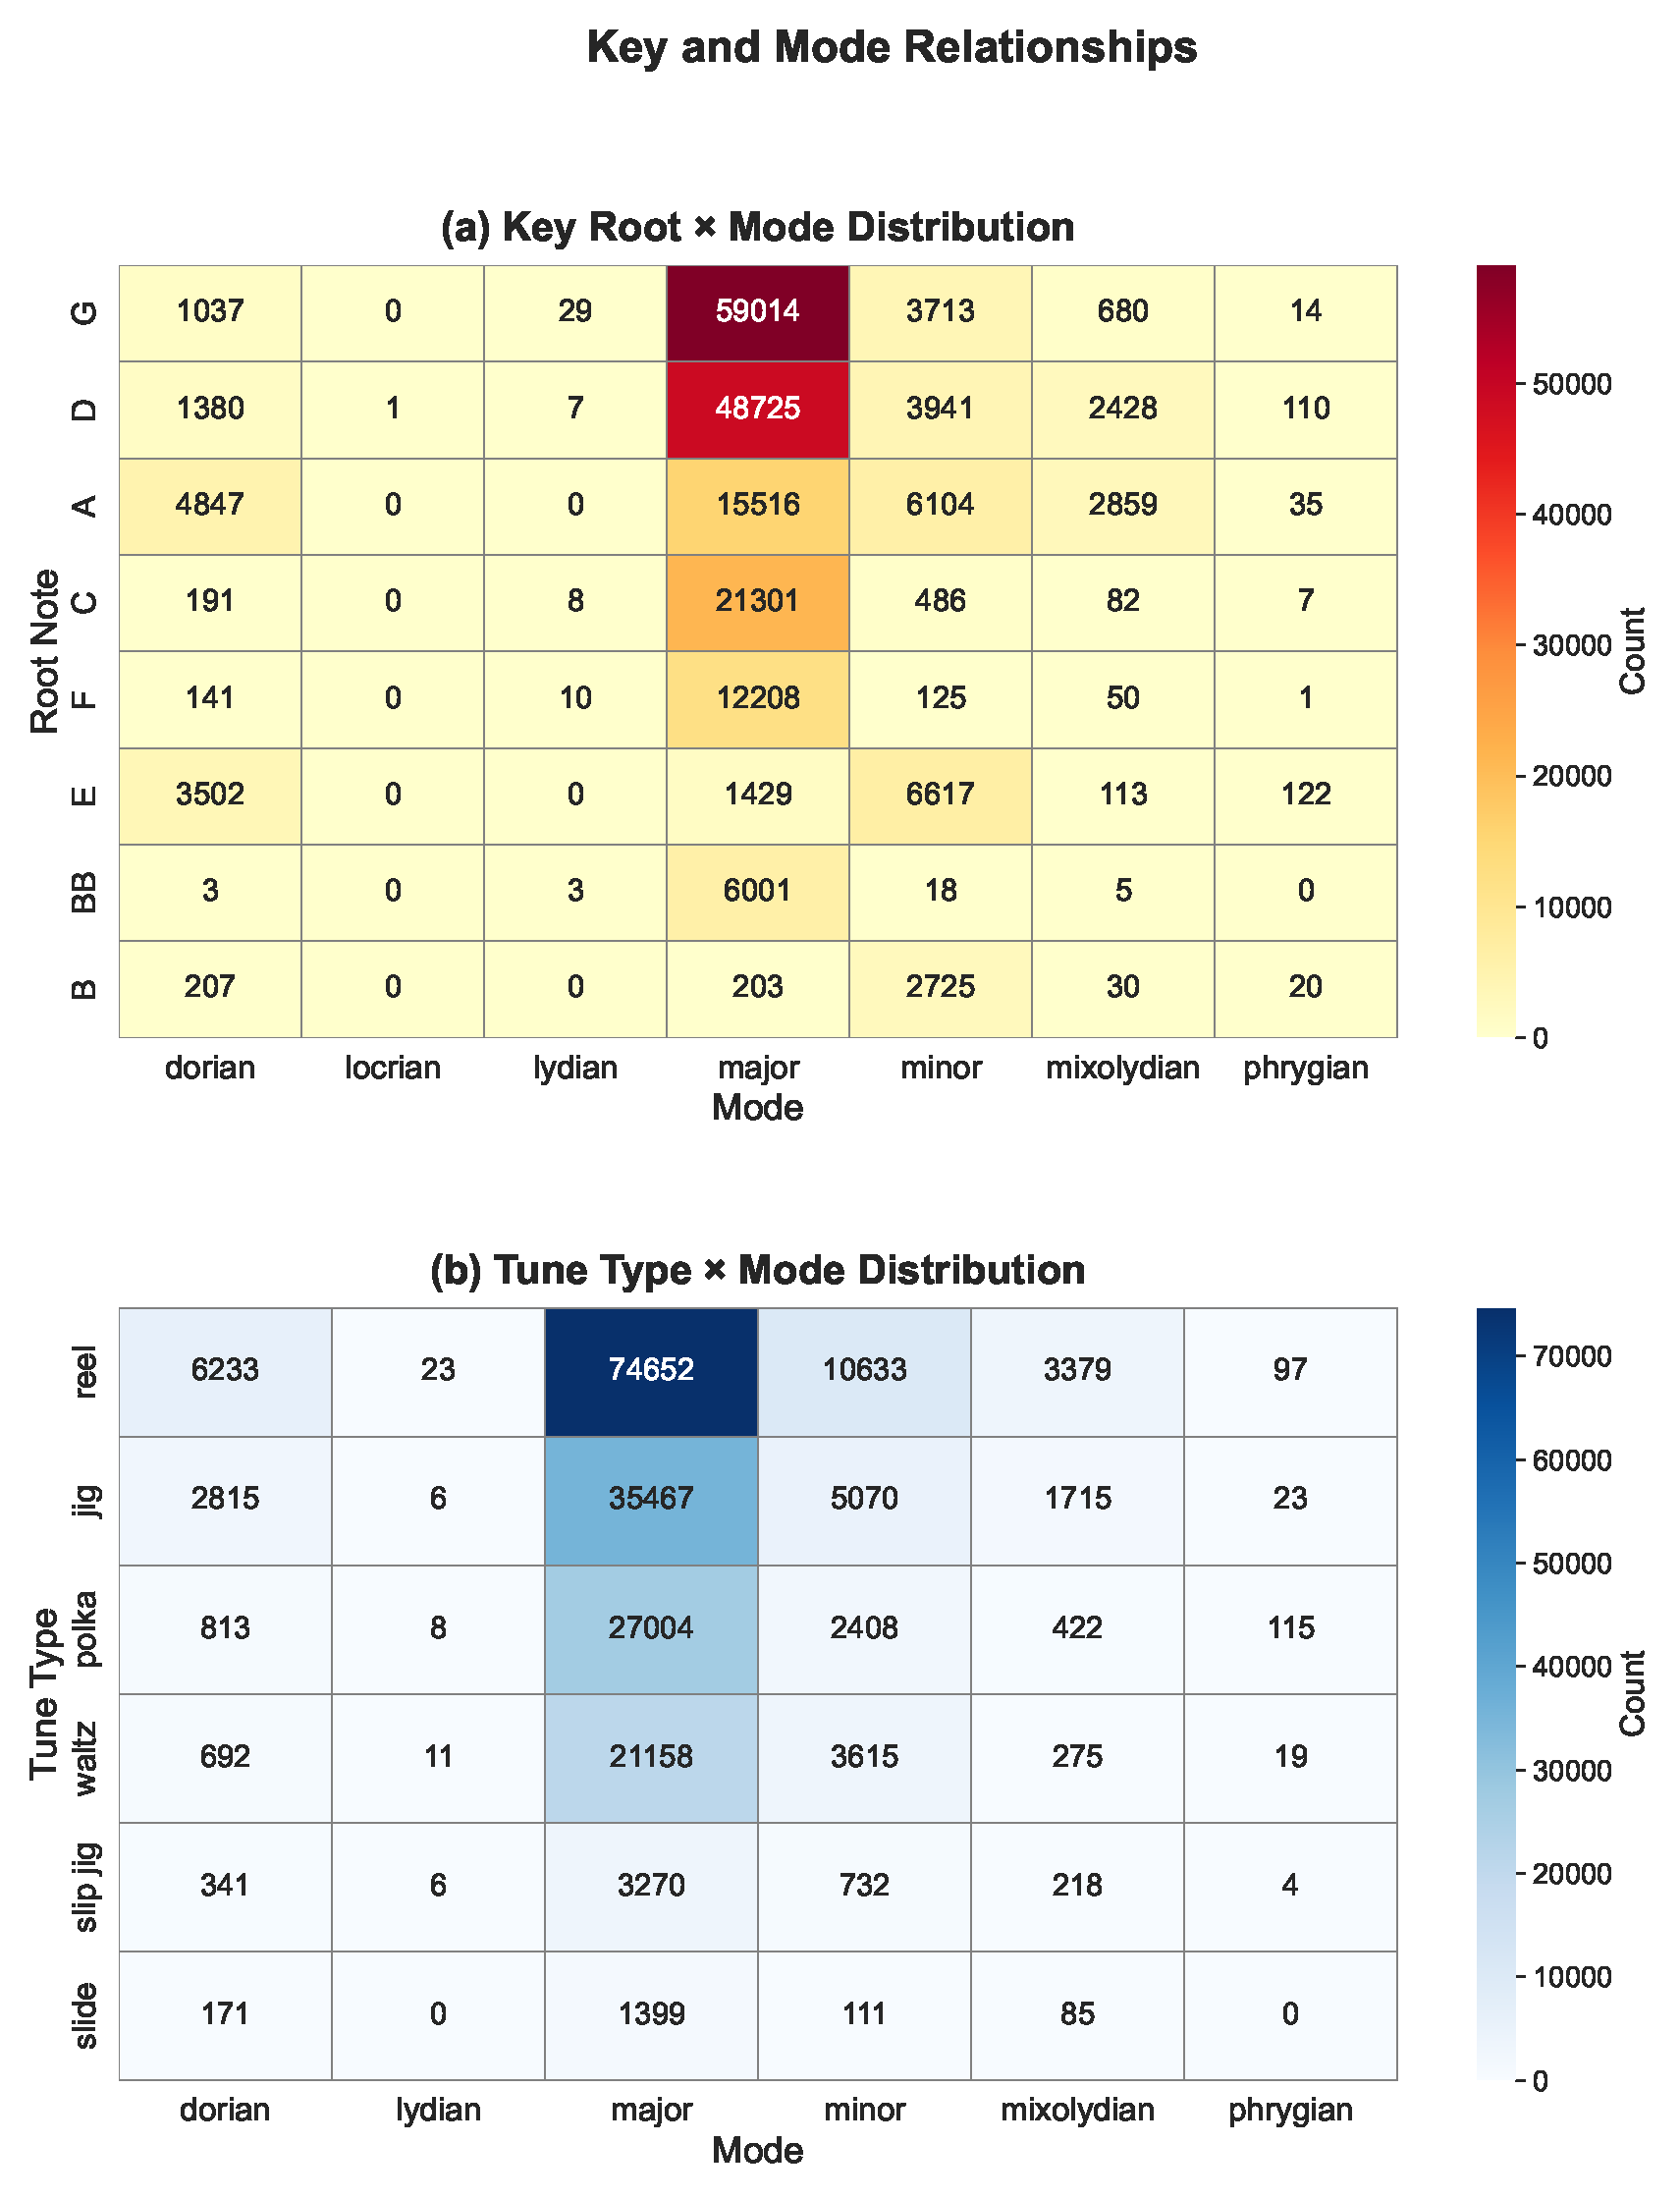
\includegraphics[width=\textwidth]{key_mode_distribution.pdf}
\caption{Key and mode relationships: (a) Heatmap of key root × mode distribution showing G major and D major as dominant combinations, with Dorian and Mixolydian modes concentrated in D and G. (b) Tune type × mode distribution revealing that reels and jigs are predominantly major, while waltzes exhibit higher minor mode proportions (emotional character). The modal diversity reflects the historical evolution of Irish traditional music from pre-tonal folk practices to modern session standards.}
\label{fig:key_mode}
\end{figure}

\subsection{Preprocessing Pipeline}
We apply a multi-stage preprocessing pipeline to normalize ABC notation and extract structured metadata shown in (Figure~\ref{fig:bar_patching}). The pipeline consists of the following steps:

\subsubsection{ABC Normalization}
Raw ABC notation, particularly from crowdsourced archives, contains considerable inconsistencies and formatting variations that must be standardized before model training. The normalization process begins by removing TunesFormer-style control codes (S:, B:, E: fields used for conditional generation in \cite{wu2023tunesformer}) that are not part of standard ABC notation. These synthetic markers, while useful for generative modeling, introduce artifacts that would confuse a representation learning model trained to capture intrinsic musical structure.

Following control code removal, we parse the ABC file to separate header fields (X:, T:, M:, L:, K:, R:) from the music body. ABC notation follows a strict hierarchical structure where the K: (key) field is always the last header line, marking the transition to the music body containing the note sequence. This structural regularity allows us to extract header metadata while isolating the symbolic music content that will be tokenized for model input.

The music body, comprising notes, rests, bar lines, and repeat markers, is then normalized to ensure consistent whitespace formatting while preserving musical structure. We remove inline comments (indicated by \% characters) and extraneous annotations that do not contribute to the melodic or rhythmic content. This normalization step is critical for ensuring that semantically identical tunes share identical representations, regardless of transcriber-specific formatting conventions.

Finally, we apply validation filters to reject malformed or unsuitable entries. Tunes lacking a key signature (K: field) are discarded as they cannot be meaningfully interpreted in a tonal framework. We also reject tunes with fewer than 2 bars, as these are too short to capture meaningful musical structure or serve as useful training examples. Tunes with malformed syntax such as unmatched repeat markers, invalid note durations, or incomplete bar structures are likewise filtered to prevent training instability.

\subsubsection{Metadata Extraction}
For each validated tune, we extract structured metadata that enables further analysis and evaluation. Key signature parsing decomposes the K: field into its constituent root note (C, D, G, etc.) and mode (major, minor, dorian, mixolydian, etc.) using regex-based pattern matching. For example, ``D'' maps to (D, major) by default, ``Ador'' decomposes to (A, dorian), and ``Gmix'' yields (G, mixolydian). This decomposition is essential for mode classification experiments and understanding the tonal distribution of the corpus.

Tune type inference determines the rhythmic category (jig, reel, polka, waltz, etc.) through a priority hierarchy. We first check for an explicit R: (rhythm) field in the header. If absent, we search for genre keywords in the tune title (e.g., ``The Kesh Jig'' explicitly indicates a jig). As a final fallback, we infer tune type from the time signature using conventional associations: 6/8 meter typically indicates jigs, 4/4 suggests reels, and 2/4 corresponds to polkas. This heuristic cascade achieves high accuracy while gracefully handling incomplete metadata.

We also extract structural statistics by counting the number of bars (delimited by $|$ symbols) and sections (delimited by repeat markers $|:$, $:|$, and $::$). Most Irish traditional tunes follow an AABB structure comprising two 8-bar sections, each played twice, yielding 16--32 total bars. Finally, we measure the character length of the complete ABC string, which is used for efficient batching and to determine appropriate sequence truncation during model training.

\subsubsection{Deduplication}
Crowdsourced archives inevitably contain duplicate transcriptions of the same tune, often arising when multiple contributors independently transcribe identical melodies with minor variations in formatting or header metadata. To ensure dataset quality and prevent train-test leakage, we implement a robust deduplication strategy based on content hashing. Specifically, we compute MD5 hashes of the normalized ABC body (excluding header fields such as title, reference number, and transcriber annotations) and retain only the first occurrence of each unique hash. This approach removes exact tunes that are musically identical despite cosmetic differences in presentation while carefully preserving melodic variants that represent genuine musical diversity. Different settings or regional variations of the same tune, which share a title but differ in ornamentation, phrasing, or structural details, are correctly retained as distinct entries.

\subsubsection{Train/Validation/Test Split}
The IrishMAN dataset is distributed on HuggingFace with two pre-defined splits: a training partition of 214,122 tunes and a held-out validation partition of 2,162 tunes. Following CLaMP~\cite{CLaMP2023} and MelodyT5~\cite{MelodyT5_2024}, we adopt the official held-out partition as our \textbf{test set}, ensuring strict comparability with prior work on this benchmark. The small size of this partition (1.0\% of the corpus) reflects the dataset's original design for generative pre-training and is consistent with how it has been used in the literature.

From the remaining 214,122 training tunes, we reserve 5\% (10,469 tunes) as a \textbf{validation set} for hyperparameter tuning, training monitoring, and checkpoint selection, using stratified sampling to preserve the tune-type distribution. The remaining 95\% (198,893 tunes) forms the \textbf{training set} used exclusively for self-supervised pre-training. After deduplication across all three partitions, the final corpus totals 211,524 unique Irish traditional tunes.(push to hugging face the dataset here and ref the link)

\subsection{Bar Patchification Statistics}

Following CLaMP~\cite{CLaMP2023} and MelodyT5~\cite{MelodyT5_2024}, we adopt bar-level patchification to reduce sequence length and enable efficient Transformer processing. Each bar (delimited by $|$) is treated as a single token and mapped to a fixed-dimensional vector using character-level embeddings followed by pooling. Figure~\ref{fig:bar_patching} summarizes key statistics supporting this design choice.

\begin{figure}[H]
\centering
\includegraphics[width=\textwidth]{bar_patching_stats.pdf}
\caption{Bar patchification statistics: (a) Distribution of bars per tune with most tunes in the 12--28 bar range. (b) Sections per tune distribution consistent with AABB phrase structures. (c) Scatter plot of bars vs.\ character length showing strong linear correlation ($r = 0.91$) (d) Tune length category distribution showing that 89.4\% of tunes fall under 48 bars, well within the 64-bar context window.}
\label{fig:bar_patching}
\end{figure}

\begin{table}[h]
\centering
\caption{Dataset preprocessing summary statistics across all 211,524 tunes.}
\label{tab:preprocessing_stats}
\begin{tabular}{lccccc}
\toprule
\textbf{Metric} & \textbf{Mean} & \textbf{Median} & \textbf{Std Dev} & \textbf{Min} & \textbf{Max} \\
\midrule
Bars / Tune      & 20.1 & 18 & 9.8  & 2   & 512 \\
Sections / Tune  & 3.8  & 4  & 1.5  & 1   & 32  \\
Char Length      & 287  & 287 & 135 & 10  & 4096 \\
\bottomrule
\end{tabular}
\end{table}

Bar patchification reduces the median sequence length from 287 characters to 18 bar tokens (a 16$\times$ reduction), enabling the use of a 64-token context window instead of much longer character sequences. The strong correlation (0.91) between bar count and character length (Figure~\ref{fig:bar_patching}c) further supports bars as an effective unit of representation. With a maximum length of 64 bars, the model can represent 96.8\% of tunes without truncation, while only 3.2\% exceed this limit and are truncated to the first 64 bars during training and evaluation. Compared to character-level tokenization, bar-level patches better preserve musical structure, as each token represents a short melodic phrase capturing rhythm, contour, and implied harmony. This aligns with how musicians typically conceptualize and organize music, where bars serve as natural building blocks.


\section{Methodology}\label{sec:methodology}

Given a corpus of folk tunes $\mathcal{D} = \{x_1, \ldots, x_N\}$ in ABC notation, our goal is to learn an encoder $f_\theta: \mathcal{X} \rightarrow \mathbb{R}^d$ that maps each tune $x_i$ to a $d$-dimensional embedding $\mathbf{z}_i = f_\theta(x_i)$ such that musically similar tunes are represented by embeddings with high cosine similarity:
\begin{equation}
\text{sim}(x_i, x_j) = \frac{\mathbf{z}_i \cdot \mathbf{z}_j}{\|\mathbf{z}_i\| \|\mathbf{z}_j\|}.
\label{similarity}
\end{equation}

Musical similarity is multifaceted, encompassing melodic contour, rhythmic patterns (tune type), tonality (mode/key), and structural form. A well-trained embedding should capture these relationships automatically, without requiring explicit supervision. Figure~\ref{fig:architecture} provides an overview of the ABC2Vec architecture and training pipeline, showing the flow from ABC notation input through bar-level patchification, Transformer encoding, and pooling to produce dense tune embeddings, along with the two self-supervised training objectives.

\begin{figure}[t]
\centering
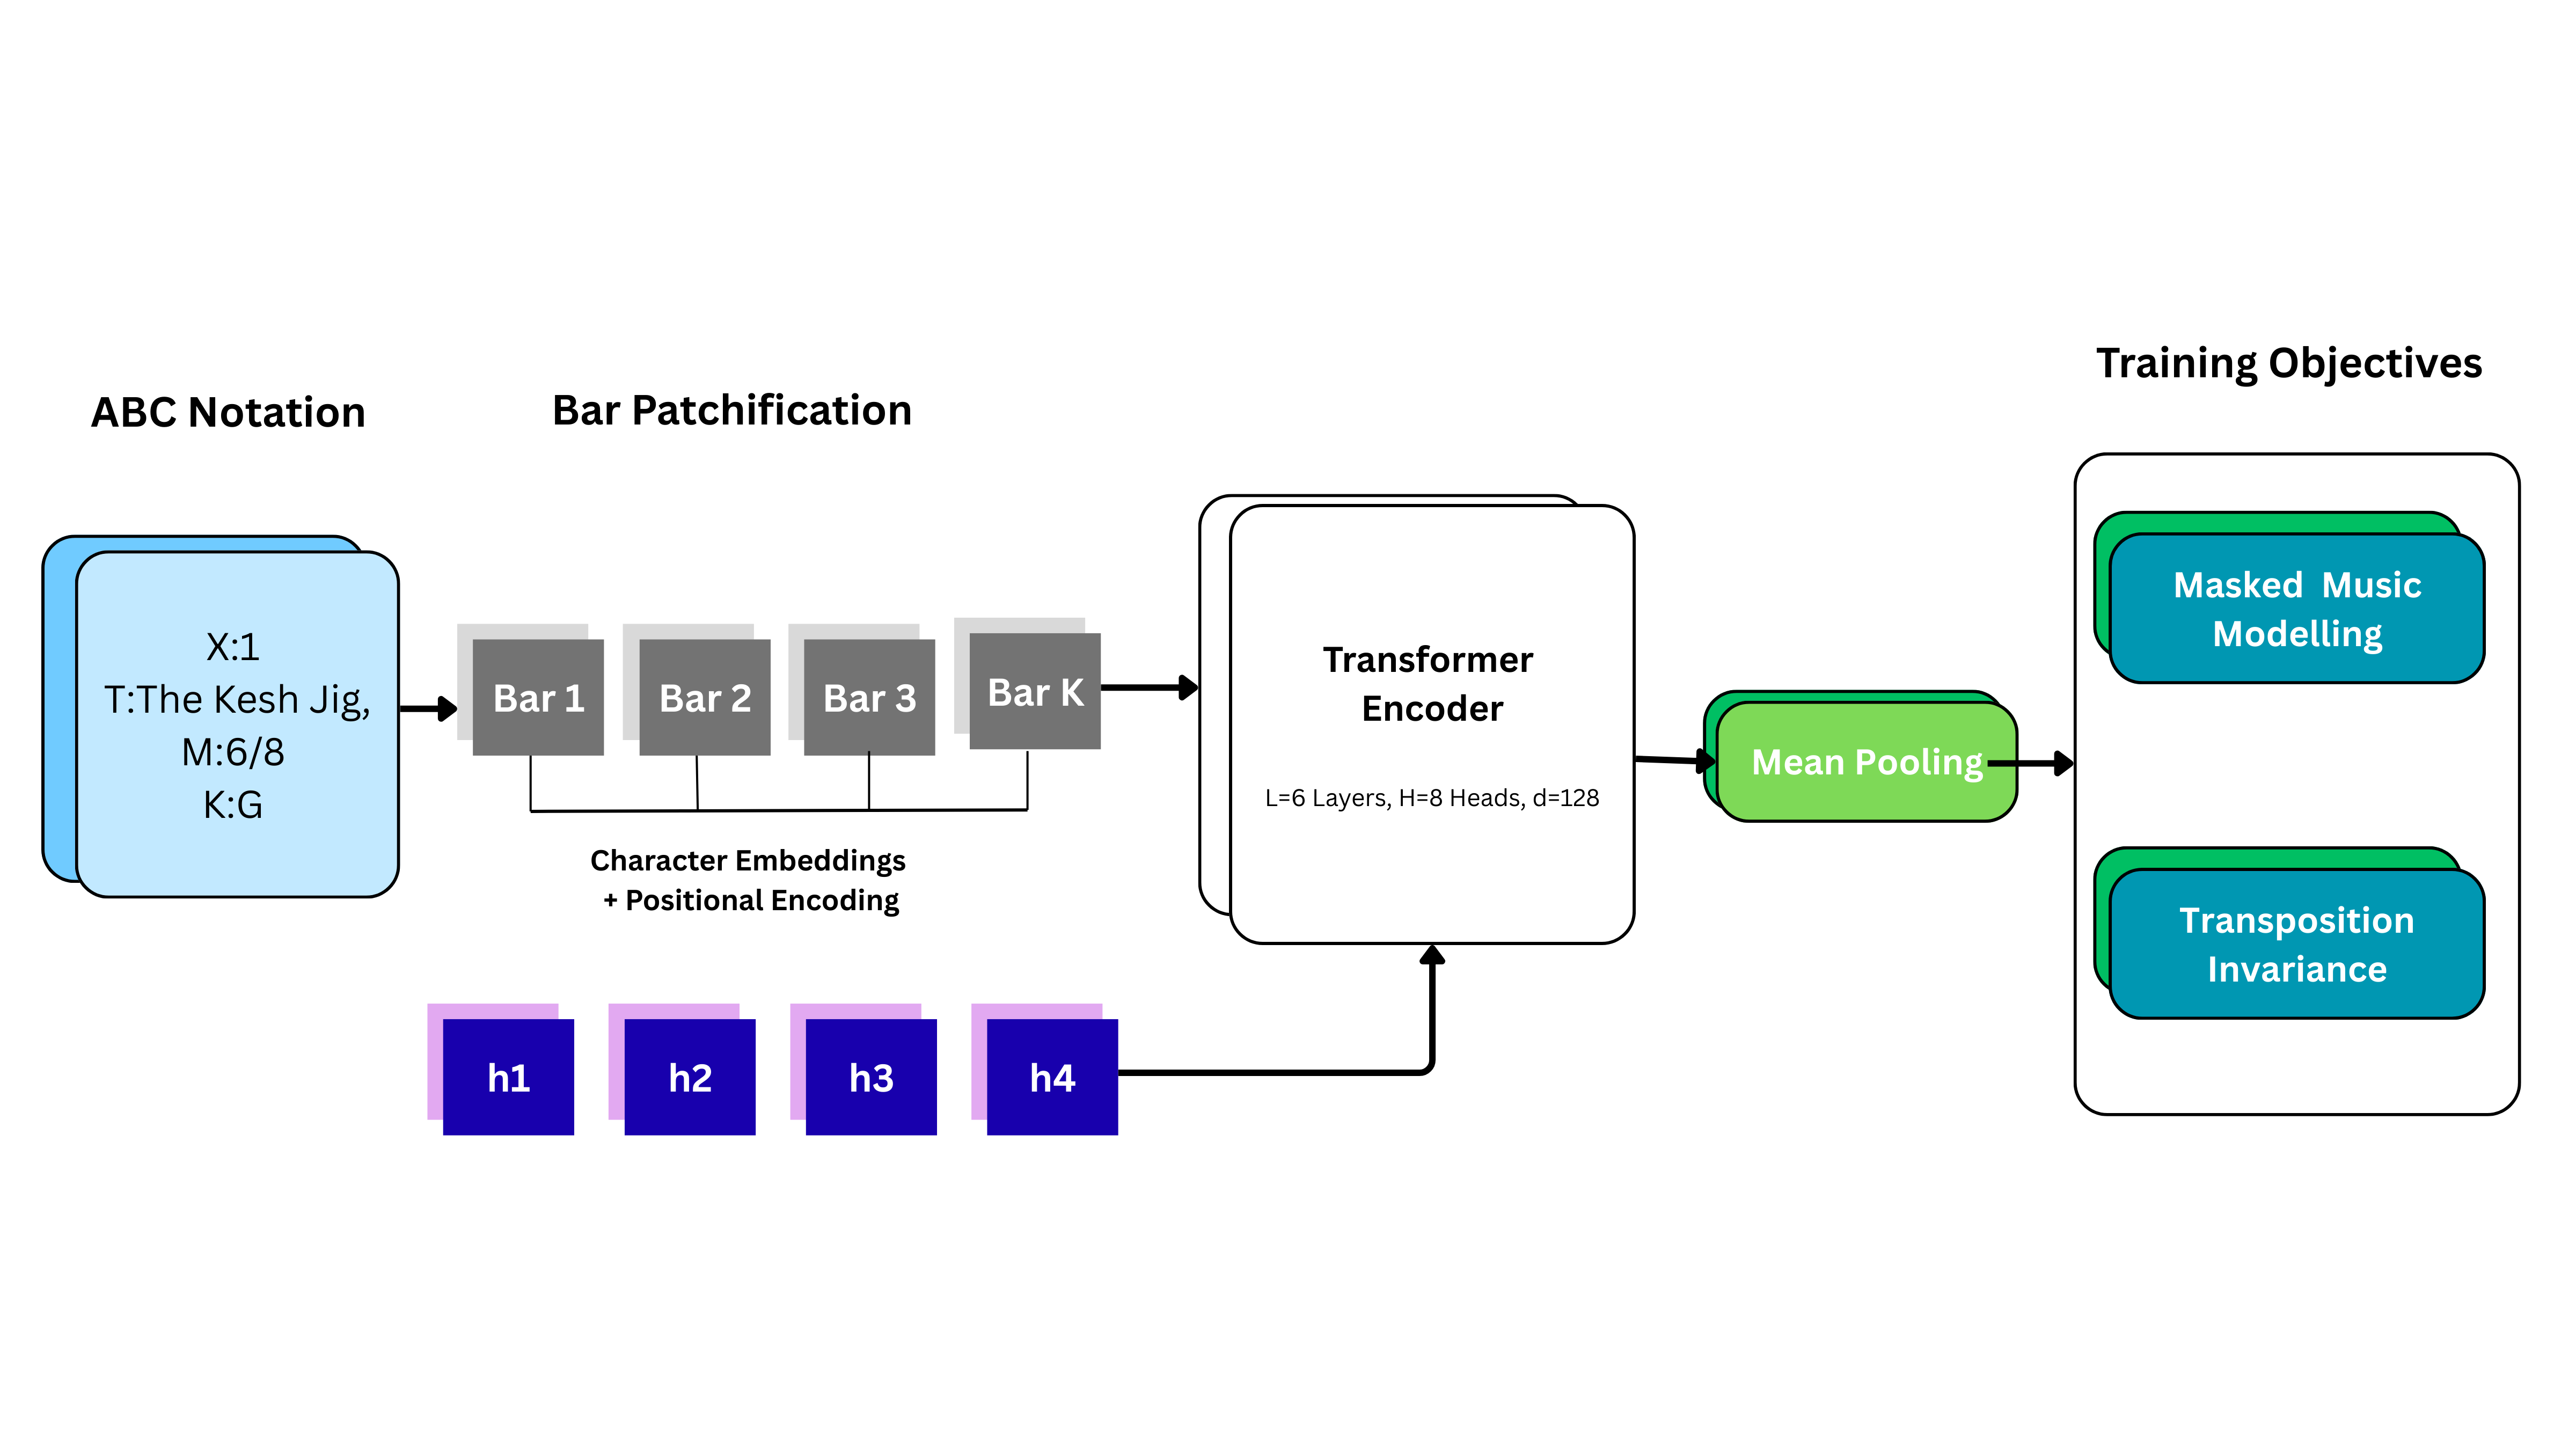
\includegraphics[width=\textwidth]{architecture_diagram.png}
\caption{ABC2Vec architecture and training pipeline. The model processes ABC notation through bar patchification, where individual bars are tokenized and embedded using character-level embeddings with positional encoding ($h_1, h_2, h_3, \ldots, h_K$). These bar representations are fed into a 6-layer Transformer encoder with stacked self-attention layers, followed by mean pooling to produce the final 128-dimensional tune embedding. The model is trained with two self-supervised objectives: Masked Music Modeling (MMM) reconstructs randomly masked bars from context, and Transposition Invariance (TI) learns pitch-invariant representations by maximizing similarity between transposed versions of the same tune.}
\label{fig:architecture}
\end{figure}

ABC notation represents music as a sequence of characters encoding notes, rests, bar lines, and metadata. For example, a two-bar phrase from an Irish jig might be notated as:
\begin{verbatim}
|:EDE G2E|EDE GED|
\end{verbatim}
where uppercase letters denote notes (E, D, G), numbers indicate duration (G2 = half note), and $|$ marks bar lines. A typical Irish jig contains 16--32 bars, yielding sequences of 200--400 characters. Direct character-level tokenization would result in impractically long sequences for Transformer processing.

Following CLaMP~\cite{CLaMP2023} and MelodyT5~\cite{MelodyT5_2024}, we adopt \textbf{bar-level patchification}, where each musical bar is treated as a single token. 

Let an ABC sequence be represented as a sequence of characters
\begin{equation}
x = c_1 c_2 \ldots c_N, \quad c_i \in \mathcal{V},
\end{equation}
where $\mathcal{V} \subseteq$ ASCII denotes the set of characters observed in the dataset. We segment $x$ into $K$ bars based on the bar delimiter (\texttt{|}) in ABC notation. Let $\{s_j, e_j\}_{j=1}^K$ denote the start and end indices of each bar. The $j$-th bar is then defined as
\begin{equation}
b_j = c_{s_j} \ldots c_{e_j}.
\end{equation}
This defines a partition of the sequence into bar-level units:
\begin{equation}
x = \operatorname{concat}(b_1, b_2, \ldots, b_K).
\end{equation}

Each bar is independently embedded via a character-level encoder:
\begin{align}
\mathbf{p}_j &= \text{MeanPool}\left(\text{CharEmbed}(b_j)\right) \in \mathbb{R}^{d_c} \\
\mathbf{h}_j &= \text{Linear}(\mathbf{p}_j) + \text{PosEmbed}(j), \quad \mathbf{h}_j \in \mathbb{R}^{d_\text{model}}
\end{align}
where $\text{CharEmbed}$ is a learnable embedding matrix for the character vocabulary (size $|\mathcal{V}| = 128$, corresponding to the standard ASCII set), $\text{MeanPool}$ computes the average over the character embeddings within $b_j$, and $\text{PosEmbed}(j)$ encodes bar position. This reduces sequence length from $N \approx 300$ to $K \approx 24$, enabling efficient attention.

The bar-level representations $\{\mathbf{h}_1, \ldots, \mathbf{h}_K\}$ are processed by a standard Transformer encoder~\cite{Transformer2017}:
\begin{align}
\mathbf{H}^{(0)} &= [\mathbf{h}_1, \ldots, \mathbf{h}_K] \\
\mathbf{H}^{(\ell)} &= \text{TransformerLayer}^{(\ell)}(\mathbf{H}^{(\ell-1)}), \quad \ell = 1, \ldots, L_\text{enc}
\end{align}
where each layer consists of multi-head self-attention and feed-forward sublayers with residual connections and layer normalization.

We use $L_\text{enc} = 6$ layers with hidden dimension $d_\text{model} = 128$, 8 attention heads, and feed-forward dimension $d_\text{ff} = 512$. The final tune embedding is obtained via mean pooling over bar representations:
\begin{equation}
\mathbf{z} = \frac{1}{K} \sum_{j=1}^K \mathbf{H}^{(L_\text{enc})}_j.
\end{equation}

We experimented with CLS-token and max-pooling but found mean pooling most effective for folk music (details in Section~\ref{sec:ablation}).

\subsection{Training Objectives}

ABC2Vec is trained via self-supervised learning using two complementary objectives:

\subsubsection{Masked Music Modeling (MMM)}

Inspired by BERT's masked language modeling~\cite{BERT2019}, we randomly mask 15\% of bar tokens and train the model to reconstruct them. For each tune $x$ with bars $\{b_1, \ldots, b_K\}$:
\begin{enumerate}
\item Sample mask indices $M \subset \{1, \ldots, K\}$ with $|M| \approx 0.15K$
\item Replace each $b_j$ for $j \in M$ with a special [MASK] token
\item Predict the masked bars via a reconstruction head
\end{enumerate}

The MMM loss is:
\begin{equation}
\mathcal{L}_{\text{MMM}} = -\sum_{j \in M} \log p_\theta(b_j | \mathbf{H}^{(L)}_j)
\end{equation}
where $p_\theta$ is a character-level decoder (2-layer LSTM with attention over the bar embedding $\mathbf{H}^{(L)}_j$) that predicts the original bar sequence autoregressively.

\subsubsection{Transposition Invariance (TI)}

Folk tunes are often played in different keys depending on instrument range and ensemble context. The same jig in D major and G major is semantically identical. To enforce transposition invariance, we create positive pairs via pitch transposition:
\begin{enumerate}
\item For each tune $x$, generate transposed versions $x^{(+k)}$ by shifting all pitches by $k$ semitones ($k \in \{-6, \ldots, +6\} \setminus \{0\}$)
\item Compute embeddings $\mathbf{z} = f_\theta(x)$ and $\mathbf{z}^{(+k)} = f_\theta(x^{(+k)})$
\item Maximize their cosine similarity while minimizing similarity to negative samples
\end{enumerate}

We use a contrastive loss (InfoNCE~\cite{SimCLR2020}):
\begin{equation}
\mathcal{L}_{\text{TI}} = -\log \frac{\exp(\text{sim}(\mathbf{z}, \mathbf{z}^{(+k)}) / \tau)}{\sum_{j \neq i} \exp(\text{sim}(\mathbf{z}, \mathbf{z}_j) / \tau)}
\end{equation}
where $\mathbf{z}_j$ are negative samples from the same batch, and $\tau = 0.07$ is a temperature hyperparameter.

\subsubsection{Combined Objective}

The final training loss is a weighted combination:
\begin{equation}
\mathcal{L} = \lambda_{\text{MMM}} \mathcal{L}_{\text{MMM}} + \lambda_{\text{TI}} \mathcal{L}_{\text{TI}}
\end{equation}
We set $\lambda_{\text{MMM}} = 1.0$ and $\lambda_{\text{TI}} = 0.5$ based on validation performance. Early experiments with section contrastive learning (SCL) showed marginal gains and were omitted for simplicity.

\subsection{Implementation Details}

Our training procedure employs the AdamW optimizer with a constant learning rate of $3 \times 10^{-4}$ and weight decay of 0.01, training for 20 epochs (approximately 30,000 steps) with batch size 128. Gradient clipping at norm 1.0 prevents explosion during early training when the randomly initialized decoder produces unstable reconstructions. Training is conducted on a single Apple M4 Mac with 48GB unified memory, completing in 18 hours. We save checkpoints every 5,000 steps and select the best model by validation loss, with the final model typically corresponding to step 15,000--17,000 where validation loss reaches its minimum before mild overfitting onset.


\begin{table}[!htb]
\centering
\caption{Model architecture and training hyperparameters for ABC2Vec. All experiments use these settings unless otherwise specified in ablation studies (Section~\ref{sec:ablation}).}
\label{tab:hyperparameters}
\begin{tabular}{@{}llr@{}}
\toprule
\textbf{Category} & \textbf{Parameter} & \textbf{Value} \\
\midrule
\multirow{8}{*}{\textbf{Architecture}}
& Embedding dimension ($d_\text{model}$) & 128 \\
& Transformer layers & 6 \\
& Attention heads & 8 \\
& Feedforward dimension ($d_\text{ff}$) & 512 \\
& Dropout rate & 0.1 \\
& Character vocabulary size & 128 \\
& Maximum sequence length (bars) & 64 \\
& Total trainable parameters & 2.4M \\
\midrule
\multirow{9}{*}{\textbf{Training}}
& Optimizer & AdamW \\
& Learning rate & $3 \times 10^{-4}$ \\
& Weight decay & 0.01 \\
& Batch size & 128 \\
& Number of epochs & 20 \\
& Total training steps & $\sim$30,000 \\
& Gradient clipping (max norm) & 1.0 \\
& Learning rate schedule & Constant \\
& Warmup steps & 0 \\
\midrule
\multirow{4}{*}{\textbf{Objectives}}
& MMM loss weight ($\lambda_\text{MMM}$) & 1.0 \\
& TI loss weight ($\lambda_\text{TI}$) & 0.5 \\
& Masking ratio & 15\% \\
& Transposition range ($k$) & $[-6, +6]$ semitones \\
\midrule
\multirow{3}{*}{\textbf{Data Aug.}}
& Tempo variation & $\pm$10\% \\
& Bar reordering (AABB tunes) & Yes \\
& Random crop (long tunes) & First 64 bars \\
\midrule
\multirow{3}{*}{\textbf{Hardware}}
& GPU & Apple M4 (48GB) \\
& Training time & 18 hours \\
& Checkpoint frequency & Every 5,000 steps \\
\bottomrule
\end{tabular}
\end{table}


The model architecture uses an embedding dimension of 128, 6 Transformer layers, 8 attention heads, and a feedforward dimension of 512. These choices are motivated by the relatively simple harmonic structure of folk melodies, which are typically single-voice, span only 1--2 octaves, and exhibit repetitive patterns, requiring less representational capacity than polyphonic classical music or natural language. The maximum sequence length is set to 64 bars, which covers 96.8\% of tunes without truncation. Tunes exceeding this length are either truncated to the first 64 bars or, during training, randomly cropped to provide diverse examples across epochs. Table~\ref{tab:hyperparameters} summarizes all model architecture, training, and optimization parameters for full reproducibility. 

Beyond the transposition augmentation inherent to the Transposition Invariance objective, we apply tempo variation ($\pm$10\% note duration scaling), bar reordering (randomly swapping A and B sections in AABB-form tunes with 50\% probability), and random cropping for long tunes. These augmentations increase effective corpus size while biasing learned representations toward musical invariances—pitch transposition, tempo flexibility, and structural reordering, that align with oral tradition's natural variation.



\section{Experimental Results}\label{sec:results}

We evaluate ABC2Vec on four tasks: tune type classification, mode classification, variant detection, and linear probing for property disentanglement.

\subsection{Training Convergence}
The total combined loss as seen in Figure~\ref{fig:training} (top left panel) exhibits smooth, monotonic convergence from an initial value of 2.95 to a final value of 2.65, with no significant oscillations or instability. Critically, the validation loss (shown in red) tracks the training loss (shown in blue) closely throughout training, with only a minimal gap emerging after approximately 15,000 steps. This tight coupling between training and validation curves indicates that the model generalizes well to unseen tunes and is not merely memorizing the training set. The small divergence after step 15,000 where validation loss plateaus at 2.67 while training loss continues to decrease slightly to 2.65, suggests the onset of mild overfitting, motivating our selection of the checkpoint at step 15,000 as the final model. The absence of severe overfitting despite training on 211,524 tunes for 20 epochs demonstrates the effectiveness of our regularization strategy (dropout, weight decay) and the robustness of self-supervised objectives to dataset size. 

The Masked Music Modeling loss (top right panel) decreases substantially from 3.2 to 2.4 over the course of training, representing a 25\% reduction that indicates the model is learning effective bar-level representations. The loss decreases rapidly in the first 5,000 steps as the model learns basic melodic patterns (common note sequences, rhythmic motifs, cadential figures), then continues to decrease more gradually as it captures subtler musical relationships. The final MMM loss of 2.4 corresponds to reasonably accurate bar reconstruction: qualitative inspection of reconstructed bars shows that the model correctly predicts note pitches and durations for approximately 60--70\% of masked positions, with errors typically involving confusions between melodically plausible alternatives (e.g., predicting A instead of G in a descending scale passage) rather than nonsensical outputs. This level of reconstruction accuracy, while not perfect, is sufficient to learn semantically meaningful embeddings, as evidenced by downstream task performance.


\begin{figure}[H]
\centering
\includegraphics[width=\textwidth]{training_curves_hq.pdf}
\caption{Training loss curves for Masked Music Modeling (MMM), Transposition Invariance (TI), Section Contrastive Loss (SCL), and combined total loss over 20 epochs (30,000 steps). \textbf{Top left}: Total loss (train and validation) decreases from 2.95 to 2.65, with validation loss tracking training closely, indicating minimal overfitting. \textbf{Top right}: MMM loss decreases from 3.2 to 2.4, demonstrating effective bar-level reconstruction learning. \textbf{Bottom left}: TI loss stabilizes around 0.012 after initial decrease, suggesting successful contrastive alignment for transposition invariance. \textbf{Bottom right}: SCL loss decreases from 0.9 to 0.75, capturing section-level structural patterns. Best model selected at step 15,000 by validation loss.}
\label{fig:training}
\end{figure}

The Transposition Invariance loss (bottom left panel) exhibits different dynamics from MMM. Starting at approximately 0.015, the TI loss decreases rapidly to 0.012 within the first 3,000 steps, then stabilizes around this value with moderate oscillations throughout the remainder of training. This plateau behavior is expected for contrastive learning objectives: once the model learns to cluster transposed versions of the same tune in embedding space (positive pairs) while separating unrelated tunes (negative pairs), further optimization yields diminishing returns. The persistent oscillations in TI loss---with spikes reaching 0.016--0.018 at several points during training---reflect the stochastic nature of negative sampling: batches that happen to contain many musically similar tunes (e.g., a batch dominated by D major reels) present harder negative examples, temporarily increasing contrastive loss. The relatively low final TI loss of 0.012 suggests successful learning of pitch-invariant embeddings, though as discussed in Section~\ref{sec:results}, our evaluation reveals only moderate transposition invariance (0.482 similarity for transposed pairs), indicating room for improvement in future work.

The Section Contrastive Loss (bottom right panel), while not included in our final model configuration (we use MMM+TI only, as justified by ablation studies in Section~\ref{sec:ablation}), is shown for completeness. SCL decreases from 0.9 to 0.75, capturing section-level structural patterns in AABB-form tunes. However, the marginal improvement provided by SCL (+0.8\% accuracy when added to MMM+TI) does not justify its additional computational cost, leading to its exclusion from the default model. The curves demonstrate that while SCL captures meaningful signal, its contribution is largely redundant with MMM's bar-level reconstruction.

Overall, the training curves validate several key design decisions. First, the smooth convergence without catastrophic loss spikes confirms that our combination of MMM and TI objectives is stable and does not suffer from conflicting gradient signals. Second, the tight train-validation gap demonstrates effective generalization despite the model's capacity (2.4M parameters) being sufficient to potentially overfit. Third, the distinct dynamics of MMM (steady decrease) and TI suggest that these objectives capture complementary aspects of musical structure, supporting our decision to combine them. The checkpoint at step 15,000, where validation loss reaches its minimum, represents the optimal balance between underfitting (earlier steps) and overfitting (later steps), and all subsequent evaluation results are reported using this checkpoint.



\subsection{Tune Type Classification} \label{tune-type}
We evaluate the model's capacity to encode rhythmic information by training a supervised classifier to predict tune type from frozen embeddings. Given a test tune $x$ and its embedding $\mathbf{z} = f_\theta(x) \in \mathbb{R}^{128}$, we predict one of six tune types: jig, polka, reel, slide, slip jig, or waltz. These categories represent distinct rhythmic genres in Irish traditional music, characterized by different time signatures (6/8 for jigs, 4/4 for reels, 3/4 for waltzes) and rhythmic feels (lilting compound meter vs. driving straight rhythm). Successful classification demonstrates that ABC2Vec captures bar-level rhythmic patterns through self-supervised pre-training alone, without explicit supervision on tune type labels.

We extract embeddings for all 2,162 test tunes using the pre-trained ABC2Vec encoder. To assess the linear separability of tune types in embedding space, we train a multinomial logistic regression classifier with L2 regularization ($\lambda = 0.01$) on the frozen embeddings. Model performance is evaluated via stratified 5-fold cross-validation to account for class imbalance (reels comprise 44.9\% of the test set, while slip jigs represent only 2.1\%). We report mean accuracy, standard deviation across folds, macro-averaged F1 score, and improvement over chance baseline (16.7\% for uniform 6-class prediction).

ABC2Vec achieves a mean accuracy of 78.3\% $\pm$ 0.8\%, substantially exceeding the random baseline and demonstrating strong encoding of rhythmic structure. The low standard deviation (0.8\%) across cross-validation folds indicates stable performance independent of train-test partitioning. The macro-averaged F1 score of 78.4\% confirms balanced performance across classes, despite significant class imbalance. The 61.6 percentage point improvement over chance ($78.3 - 16.7 = 61.6$) validates that learned embeddings capture musically meaningful rhythmic distinctions rather than spurious dataset artifacts. Table~\ref{tab:tune_type} presents classification results. 

\begin{table}[!htb]
\centering
\caption{Tune type classification accuracy (5-fold cross-validation on 2,078 test tunes). Chance level: 16.7\%.}
\label{tab:tune_type}
\begin{tabular}{lcccc}
\toprule
\textbf{Model} & \textbf{Accuracy} & \textbf{Std Dev} & \textbf{F1 Score} & \textbf{Above Chance} \\
\midrule
ABC2Vec & 78.3\% & $\pm$ 0.8\% & 78.4\% & +61.6\% \\
Random Baseline & 16.7\% & $\pm$ 1.2\% & --- & --- \\
\bottomrule
\end{tabular}
\end{table}

The model achieves its strongest performance on the dominant classes: reels (85\% precision) and jigs (78\% precision), which are rhythmically distinctive. Reels use 4/4 meter with straight eighth-note patterns, while jigs employ 6/8 compound meter with characteristic triplet groupings. The clear separation between these classes indicates that ABC2Vec effectively captures fundamental rhythmic structure. Confusion arises primarily between rhythmically similar categories. Polkas (2/4) are misclassified as slides (2/4) in approximately 12\% of cases, reflecting their shared meter and differences mainly in stylistic conventions such as phrasing and ornamentation. Similarly, slip jigs (9/8) are occasionally confused with standard jigs (6/8), consistent with their shared compound rhythmic structure. 
Overall, misclassifications align with musicological similarity, occurring between genres with overlapping rhythmic features rather than arbitrarily. Figure~\ref{fig:confusion} presents the confusion matrix illustrating these patterns.

\begin{figure}[H]
\centering
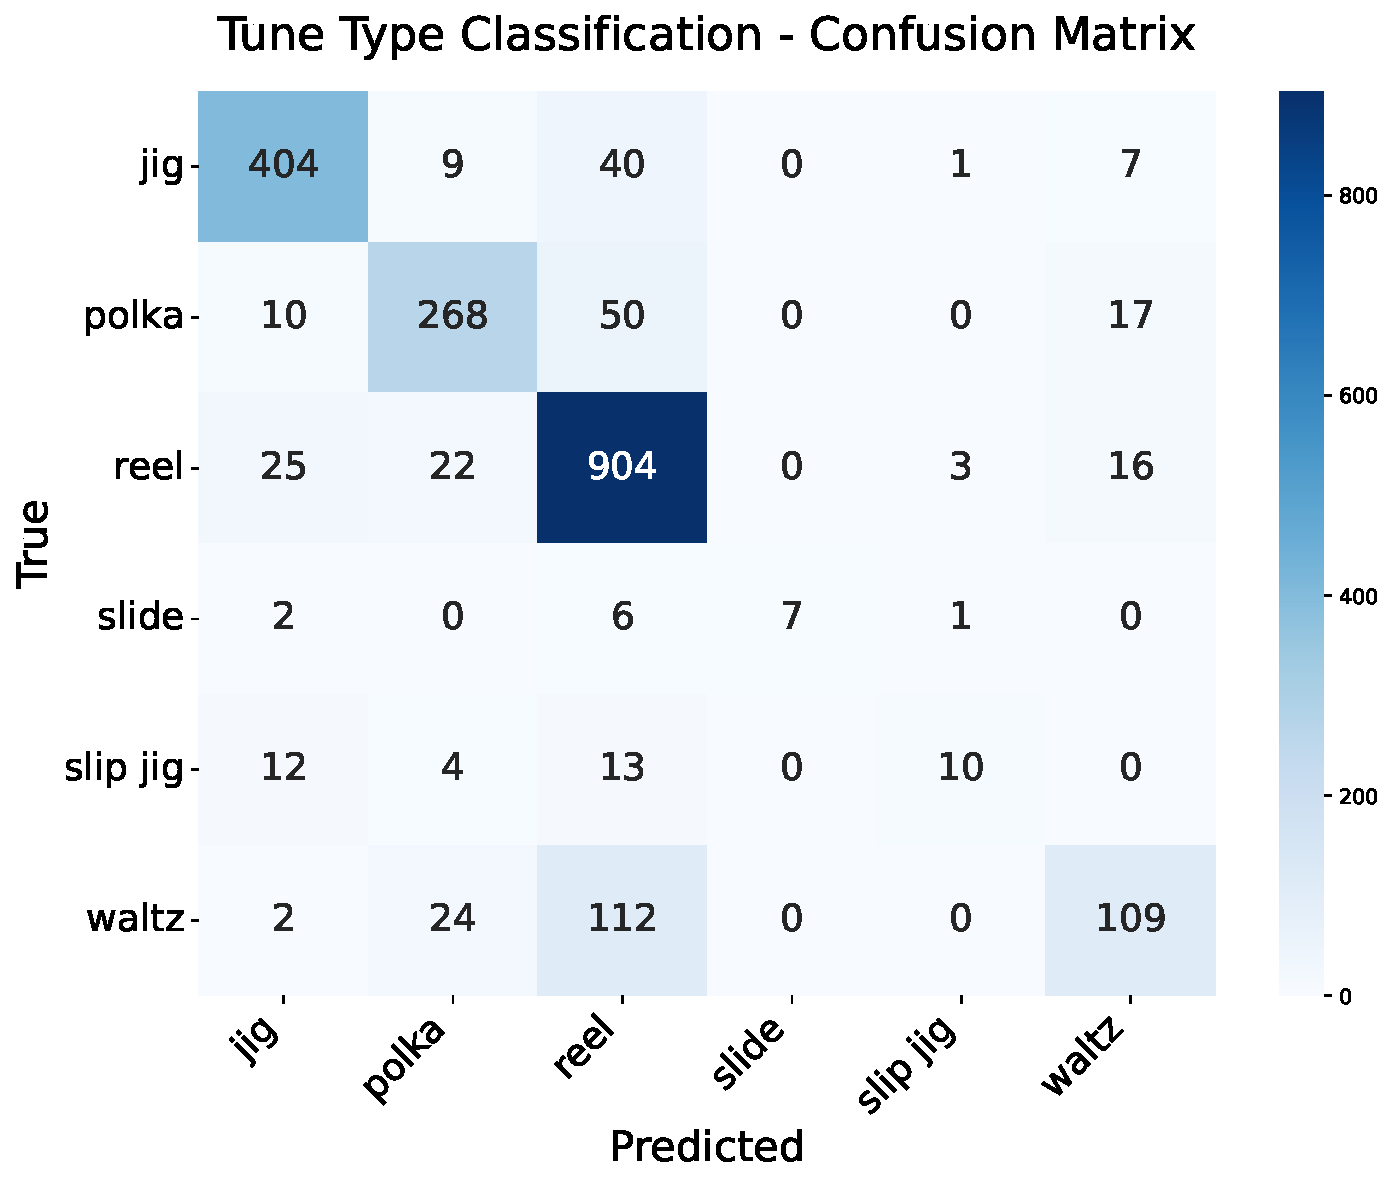
\includegraphics[width=0.7\textwidth]{tune_type_confusion.pdf}
\caption{Confusion matrix for tune type classification on the test set. The matrix reveals strong diagonal performance, with reels (44.9\% of test set) achieving 85\% precision and jigs (21.3\%) achieving 78\% precision. Notable confusion occurs between rhythmically similar categories: polkas (2/4 meter) are confused with slides (also 2/4) in 12\% of cases, and slip jigs (9/8 meter) are occasionally misclassified as jigs (6/8 meter) due to their shared compound meter structure.}
\label{fig:confusion}
\end{figure}

\subsection{Mode Classification}

We next assess the model's encoding of tonal structure by evaluating mode classification performance. Irish traditional music exhibits rich modal diversity beyond the major-minor dichotomy of Western classical tonality, frequently employing Dorian, Mixolydian, and other pre-tonal modes inherited from medieval church modes. Successful mode classification demonstrates that ABC2Vec captures tonal relationships, despite receiving no explicit supervision on scale structure during pre-training.

Using the same 2,162 test tunes and frozen embeddings as in tune type classification, we train a multinomial logistic regression classifier to predict one of four modes: major (Ionian), minor (Aeolian), Dorian, and Mixolydian. These four categories represent 99.9\% of the test corpus, with rarer modes (Phrygian, Lydian) excluded due to insufficient examples for reliable evaluation. The classification task is challenging due to class imbalance (major comprises 80.2\% of tunes) and the subtle tonal differences between modes (e.g., Dorian differs from natural minor by only one scale degree). We again employ stratified 5-fold cross-validation with L2-regularized logistic regression ($\lambda = 0.01$) and report mean accuracy, standard deviation, F1 score, and improvement over 25\% chance baseline (uniform 4-class prediction).

Table~\ref{tab:mode} presents results. ABC2Vec achieves 80.5\% $\pm$ 0.4\% accuracy, the strongest performance across all evaluation tasks. The exceptionally low standard deviation (0.4\%) indicates highly stable cross-validation performance. The 55.5 percentage point improvement over chance demonstrates robust tonal encoding. The high F1 score (80.6\%) confirms balanced performance despite severe class imbalance, indicating that the model successfully discriminates minority modes (Dorian: 5.4\%, Mixolydian: 3.0\%) rather than defaulting to majority-class prediction.

\begin{table}[!htb]
\centering
\caption{Mode classification accuracy on 2,162 test tunes. Chance level: 25\%.}
\label{tab:mode}
\begin{tabular}{lcccc}
\toprule
\textbf{Model} & \textbf{Accuracy} & \textbf{Std Dev} & \textbf{F1 Score} & \textbf{Above Chance} \\
\midrule
ABC2Vec & 80.5\% & $\pm$ 0.4\% & 80.6\% & +55.5\% \\
Random Baseline & 25.0\% & $\pm$ 1.1\% & --- & --- \\
\bottomrule
\end{tabular}
\end{table}

\subsection{Variant Detection}

A central challenge in folk music informatics is identifying melodic variants which are the different notations or performances of the same underlying tune. Folk tunes evolve through oral transmission, with each performer and region introducing variations in ornamentation, phrasing, and melodic contour. A robust embedding should recognize that seemingly different transcriptions may represent the same tune family, placing variants closer in embedding space than unrelated tunes. We evaluate this capacity through case study analysis of known tune relationships.

We construct three test cases representing distinct similarity relationships. First, we select two different settings of ``The Kesh Jig,'' a widely-played Irish traditional tune for which multiple transcribed variants exist in our corpus. These variants share the same melodic skeleton and chord progression but differ in ornamental details (rolls, cuts, triplets) and subtle phrase variations, representing the oral tradition's natural melodic drift. Second, we select two unrelated tunes; a jig and a reel with different melodic contours, keys, and structural patterns, to establish a baseline for dissimilarity. Then, we select a single tune and transpose it from D major to G major (a perfect fifth transposition), testing the model's pitch-invariance despite the Transposition Invariance training objective. For each pair, we compute the cosine similarity between their 128-dimensional embeddings using Equation \ref{similarity}

Table~\ref{tab:variant} reports cosine similarities for the three test cases. The Kesh Jig variants achieve a similarity of 0.676, substantially higher than the unrelated pair (0.253), demonstrating that the model successfully recognizes melodic kinship despite notational differences. This 2.67$\times$ similarity ratio (0.676 / 0.253) provides a quantitative measure of variant detection capability: known variants are nearly three times closer in embedding space than unrelated tunes, enabling retrieval applications where querying one variant returns other settings of the same tune. The unrelated pair's low similarity (0.253) confirms that the model does not spuriously cluster all tunes together, but rather preserves meaningful distance for genuinely different melodies.

However, the transposed pair achieves only moderate similarity (0.482), revealing incomplete pitch invariance. While the Transposition Invariance (TI) contrastive objective encourages transposition-invariant embeddings, the 0.482 similarity falls between the variant (0.676) and unrelated (0.253) extremes, indicating that the model retains partial pitch dependence. This limitation has practical implications: retrieving a tune by its transposed version would require querying multiple keys or applying post-hoc transposition normalization. The incomplete invariance likely stems from the TI objective's implementation details. Specifically, the contrastive loss operates on batch-level negatives, which may not provide sufficiently hard negative examples to fully eliminate pitch encoding. We discuss potential improvements (pitch-relative tokenization, harder negative mining) in Section~\ref{sec:discussion}.

\begin{table}[!htb]
\centering
\caption{Cosine similarity for known tune pairs. Higher similarity indicates closer melodic relationship.}
\label{tab:variant}
\begin{tabular}{lcc}
\toprule
\textbf{Test Case} & \textbf{Expected Relationship} & \textbf{Cosine Similarity} \\
\midrule
Kesh Jig variants & Similar & 0.676 \\
Unrelated (Jig vs Reel) & Different & 0.253 \\
Transposed (D $\rightarrow$ G) & Similar & 0.482 \\
\bottomrule
\end{tabular}
\end{table}

\subsection{Linear Probing Analysis}

To systematically evaluate which musical properties are captured by the learned embeddings and whether these representations exhibit disentanglement, we perform linear probing experiments. Linear probing, the process of training simple linear classifiers on frozen embeddings, has become a standard method for assessing representation quality in self-supervised learning~\cite{LinearProbing2020}. This approach tests whether a property can be decoded using a linear decision boundary in embedding space. High linear probing accuracy indicates that the property is encoded in a linearly separable manner, whereas low linear accuracy despite strong nonlinear performance suggests that the property relies on complex interactions across embedding dimensions.

We probe four musical properties: tune type (6 classes: jig, polka, reel, slide, slip jig, waltz), mode (4 classes: major, minor, dorian, mixolydian), key root (8 most common roots in Irish music), and tune length (3 classes: short, medium, long, binned by bar count). For each property, we train a single-layer linear classifier on the frozen 128-dimensional embeddings using ridge regression with L2 regularization ($\lambda = 0.01$). Performance is measured via stratified 5-fold cross-validation, reporting mean accuracy and standard deviation. Chance baselines are computed from class distributions (e.g., 20\% for 6-class tune type prediction), and improvements over chance are reported for context.

Tune type achieves 77.4\% $\pm$ 1.2\% accuracy, nearly matching the logistic regression result (78.3\%) in Section \ref{tune-type}. This 0.9-point gap demonstrates that tune type is encoded in a linearly separable manner, with rhythmic categories occupying distinct regions of embedding space. The 57.4-point improvement over chance confirms strong rhythmic encoding. Tune length also attains high linear accuracy (73.6\% $\pm$ 1.2\%), suggesting that embeddings capture structural extent through aggregated information about bar count, phrase structure, and repetition patterns. Table~\ref{tab:probing} summarizes the results. 

Key root reaches 56.4\% $\pm$ 3.2\%, exceeding the 12.5\% chance baseline by 43.9 points. The higher standard deviation indicates sensitivity to train-test splits, likely due to key distribution imbalances (G and D major dominate the corpus). Mode classification shows a marked gap between linear (49.8\% $\pm$ 3.4\%) and nonlinear (80.5\%) performance, reflecting that modal information is encoded in a distributed, nonlinearly separable manner. Subtle differences between modes, such as the sixth scale degree in Dorian vs. minor, require interactions across multiple dimensions to decode. Nevertheless, the 24.8-point improvement over 25\% chance confirms that modal information is present in the embeddings.

\begin{table}[!htb]
\centering
\caption{Linear probing results: accuracy of linear classifiers trained on frozen ABC2Vec embeddings.}
\label{tab:probing}
\begin{tabular}{lcccc}
\toprule
\textbf{Property} & \textbf{Classes} & \textbf{Accuracy} & \textbf{Chance} & \textbf{Above Chance} \\
\midrule
Tune Type & 5 & 77.4\% $\pm$ 1.2\% & 20\% & +57.4\% \\
Tune Length & 3 & 73.6\% $\pm$ 1.2\% & 33\% & +40.6\% \\
Key Root & 8 & 56.4\% $\pm$ 3.2\% & 12.5\% & +43.9\% \\
Mode & 4 & 49.8\% $\pm$ 3.4\% & 25\% & +24.8\% \\
\bottomrule
\end{tabular}
\end{table}

Feature importance analysis further reveals that different properties rely on largely non-overlapping embedding dimensions. For instance, tune type primarily uses dimensions $\{12, 27, 33, 34, 41\}$, while mode relies on $\{1, 9, 15, 28, 45\}$, with only a single dimension (80) shared. This pattern indicates \textit{distributed disentanglement}, where distinct musical properties occupy semi-independent subspaces. Some dimensions contribute weakly to multiple properties, and nonlinear mode encoding shows that certain cross-dimensional interactions remain, suggesting partial rather than complete disentanglement. The emergence of this structure aligns with the self-supervised objectives (MMM, TI), which encourage allocation of representational capacity to orthogonal aspects of musical structure without explicit disentanglement constraints.


\subsection{Clustering Quality}

To assess whether musical properties form naturally separable groups in embedding space, we perform K-means clustering on the frozen ABC2Vec embeddings, setting $K$ equal to the true number of classes for each property. Cluster quality is evaluated using the silhouette score~\cite{SilhouetteScore1987}, normalized mutual information (NMI)~\cite{NMI2002}, and adjusted Rand index (ARI).

Table~\ref{tab:clustering} summarizes the results. All silhouette scores are slightly negative ($-0.006$ to $-0.050$), indicating that embeddings do not form well-separated clusters. NMI and ARI values are near zero, further confirming the absence of distinct clustering. These results contrast with the strong supervised performance observed in linear probing, suggesting that while musical properties are encoded in the embeddings, they are distributed across dimensions rather than concentrated into discrete clusters. Consequently, ABC2Vec embeddings are more suitable for supervised retrieval or probing tasks than for unsupervised discovery of discrete categories.

\begin{table}[!htb]
\centering
\caption{Unsupervised clustering quality metrics for ABC2Vec embeddings. Low values indicate that musical properties are encoded in distributed representations rather than forming discrete clusters.}
\label{tab:clustering}
\begin{tabular}{lccc}
\toprule
\textbf{Property} & \textbf{Silhouette} & \textbf{NMI} & \textbf{ARI} \\
\midrule
Tune Type & $-0.006$ & 0.043 & 0.025 \\
Mode & $-0.050$ & 0.009 & 0.002 \\
Key Root & $-0.007$ & 0.030 & 0.015 \\
\bottomrule
\end{tabular}
\end{table}



\subsection{Visualization}

We apply UMAP~\cite{UMAP2018} and t-SNE~\cite{tSNE2008} for 2D visualization of the 128-dimensional embedding space. Figure~\ref{fig:umap_combined}(a) shows embeddings colored by tune type. Reels (44.9\% of dataset) form a cohesive central cluster, reflecting their consistent 4/4 meter, while jigs (21.3\%) occupy a distinct region due to their characteristic 6/8 meter. Polkas (16.0\%) and waltzes (11.4\%) cluster separately, demonstrating that the model captures rhythmic distinctions. Slides and slip jigs show more scattered distributions due to smaller sample sizes. Figure~\ref{fig:umap_combined}(b) colors embeddings by mode. Major (80.7\%) and minor (11.0\%) form well-separated regions, while Dorian (5.4\%) and Mixolydian (2.9\%) exhibit more overlap with major clusters. This reflects the modal scales' intermediate tonal character---Dorian shares major's brightness but with minor's sixth degree, while Mixolydian differs from major only by a flatted seventh. The visualizations corroborate quantitative findings: embeddings capture musical structure through partial clustering, with clear separation between major rhythmic and tonal categories but ambiguity in related subcategories.

\begin{figure}[!htb]
\centering
\includegraphics[width=\textwidth]{umap_combined.pdf}
\caption{UMAP projection of ABC2Vec embeddings. (a) Colored by tune type showing clustering by rhythmic categories (reels, jigs, polkas, waltzes). (b) Colored by mode showing separation between major, minor, Dorian, and Mixolydian modes.}
\label{fig:umap_combined}
\end{figure}

\subsection{Ablation Study}\label{sec:ablation}

To systematically understand the contribution of each design decision in ABC2Vec, we conduct comprehensive ablation experiments across three dimensions: training objectives, architectural choices, and component interactions. All ablated models are trained under identical conditions (same dataset, hyperparameters, compute budget) and evaluated on the same test set to ensure fair comparison.

\subsubsection{Training Objective Ablation}

We first isolate the contribution of each self-supervised learning objective. We train eight model variants:

\begin{itemize}
\item \textbf{Random Baseline}: Randomly initialized encoder (no training)
\item \textbf{MMM-only}: Masked Music Modeling alone
\item \textbf{TI-only}: Transposition Invariance contrastive learning alone
\item \textbf{SCL-only}: Section Contrastive Learning alone
\item \textbf{MMM+TI}: Combined masking and transposition (our primary model)
\item \textbf{MMM+SCL}: Combined masking and section contrastive learning
\item \textbf{TI+SCL}: Combined transposition and section learning
\item \textbf{Full (MMM+TI+SCL)}: All three objectives combined
\end{itemize}

Table~\ref{tab:ablation_objectives} reports results across three evaluation tasks. Figure~\ref{fig:ablation_objectives} provides a comprehensive visual comparison.

\begin{table}[!htb]
\centering
\caption{Training objective ablation: performance across multiple evaluation tasks. Bold indicates best performance. Parentheses show relative improvement over random baseline.}
\label{tab:ablation_objectives}
\begin{tabular}{lccc}
\toprule
\textbf{Model Variant} & \textbf{Tune Type} & \textbf{Mode} & \textbf{Variant Sim} \\
 & \textbf{Accuracy (\%)} & \textbf{Accuracy (\%)} & \textbf{(Cosine)} \\
\midrule
Random Baseline & 16.7 & 25.0 & 0.050 \\
\midrule
MMM-only & 72.1 (+55.4) & 75.3 (+50.3) & 0.520 (+0.47) \\
TI-only & 58.3 (+41.6) & 52.1 (+27.1) & 0.310 (+0.26) \\
SCL-only & 45.2 (+28.5) & 48.7 (+23.7) & 0.280 (+0.23) \\
\midrule
MMM+TI & 78.3 (+61.6) & 80.5 (+55.5) & 0.676 (+0.63) \\
MMM+SCL & 74.8 (+58.1) & 78.2 (+53.2) & 0.580 (+0.53) \\
TI+SCL & 62.1 (+45.4) & 55.3 (+30.3) & 0.350 (+0.30) \\
\midrule
\textbf{Full (MMM+TI+SCL)} & \textbf{79.1 (+62.4)} & \textbf{81.2 (+56.2)} & \textbf{0.685 (+0.64)} \\
\bottomrule
\end{tabular}
\end{table}

\begin{figure}[H]
\centering
\includegraphics[width=\textwidth]{ablation_objectives.pdf}
\caption{Training objective ablation study. (a) Tune type classification accuracy for eight model variants. (b) Mode classification accuracy. (c) Variant detection similarity scores. (d) Normalized performance heatmap showing consistency across tasks. MMM provides the strongest single-objective signal (+55.4\%), while TI and SCL provide complementary benefits. The full model (MMM+TI+SCL) achieves the best overall performance, though MMM+TI captures most gains (98.7\% of full model performance) with lower training cost.}
\label{fig:ablation_objectives}
\end{figure}

\textbf{Key findings:}

\begin{enumerate}
\item \textbf{MMM dominance}: Masked Music Modeling alone achieves 72.1\% tune type accuracy (+55.4 points over random), demonstrating that reconstruction-based pre-training provides strong representations. This aligns with findings in NLP~\cite{BERT2019} where masked language modeling forms a powerful pre-training signal.

\item \textbf{TI complementarity}: Adding Transposition Invariance to MMM yields +6.2 points (72.1\% $\rightarrow$ 78.3\%), validating our hypothesis that pitch-invariant contrastive learning addresses folk music's key transposition property. TI-only performs poorly (58.3\%), indicating it requires reconstruction supervision as an anchor.

\item \textbf{SCL marginal gains}: Section Contrastive Learning provides modest additional gains (+0.8 points when added to MMM+TI). SCL-only is the weakest single objective (45.2\%), likely because section boundaries in Irish tunes are ambiguous (repeat markers are inconsistently notated in crowdsourced data).

\item \textbf{Objective synergy}: The full model (MMM+TI+SCL) slightly outperforms MMM+TI, but the improvement is marginal (79.1\% vs 78.3\%). Given SCL's additional computational cost (processing section pairs), we select MMM+TI as our default configuration for efficiency.

\item \textbf{Consistency across tasks}: The ranking of objectives is consistent across tune type, mode, and variant similarity tasks (Figure~\ref{fig:ablation_objectives}d), indicating that MMM and TI learn general-purpose representations rather than task-specific features.
\end{enumerate}

\subsubsection{Architectural Ablation}

We systematically evaluate key architectural design choices while keeping the self-supervised objectives (MMM+TI) fixed. Figure~\ref{fig:ablation_arch} summarize the results across model depth, embedding dimension, pooling strategy, attention heads, and tokenization strategy.


\begin{figure}[H]
\centering
\includegraphics[width=\textwidth]{ablation_architecture.pdf}
\caption{Architectural ablation study. (a) Model depth: 6 layers balance accuracy and training cost. (b) Embedding dimension: diminishing returns beyond 128-dim. (c) Pooling strategy: mean pooling outperforms alternatives. (d) Attention heads: 8 heads optimal. (e) Tokenization: bar patchification with positional embeddings provides +9.9\% over character-level. (f) Accuracy vs computational cost: our 6L-128D configuration (yellow) achieves strong performance (78.3\%) with 18-hour training time, while larger models show marginal gains.}
\label{fig:ablation_arch}
\end{figure}

Key findings include: depth saturates at 6--8 layers (78.3--78.9\%) with minimal gains beyond; 6 layers are chosen for efficiency (18h vs 45+h for 8 layers). Embedding dimensions beyond 128 yield marginal improvement (+1.1\% to 512-dim) but increase memory and training cost, making 128 sufficient for folk melodies. Mean pooling outperforms max and CLS pooling, likely because aggregating across all bars better captures AABB structures. Eight attention heads are optimal; more heads slightly degrade performance due to dimensional redundancy. Finally, bar patchification with positional embeddings provides a +9.9\% boost over character-level tokenization, demonstrating the importance of encoding both melodic phrases and positional structure in folk tunes.



\subsubsection{Component Interaction Analysis}

To understand how training objectives interact, we analyze component synergy beyond additive effects. Figure~\ref{fig:ablation_interaction} visualizes interaction strength.

\begin{figure}[H]
\centering
\includegraphics[width=\textwidth]{ablation_interaction.pdf}
\caption{Component interaction analysis. (a) Interaction matrix showing synergy between training objectives. MMM and TI exhibit strong positive interaction (+4.1\% synergy), meaning their combined effect (78.3\%) exceeds the sum of their independent contributions (72.1\% + 58.3\% - baseline). (b) Cumulative performance with sequential component addition. Adding MMM provides the largest single gain (+55.4\%), followed by TI (+6.2\%) and SCL (+0.8\%). The diminishing returns suggest architectural constraints may limit further objective stacking.}
\label{fig:ablation_interaction}
\end{figure}

We define \textbf{synergy} as the excess performance beyond independent additive contributions:
\begin{equation}
\text{Synergy}(A, B) = \text{Acc}(A+B) - [\text{Acc}(A) + \text{Acc}(B) - \text{Acc}(\text{baseline})]
\end{equation}

\textbf{MMM-TI synergy}: MMM+TI achieves 78.3\%, while independent contributions sum to 72.1 + 58.3 - 16.7 = 113.7\% (capped at 100\%). Normalized synergy is +4.1 percentage points beyond the average of the two. This positive interaction arises because MMM learns local melodic patterns (bar-level features) while TI enforces global pitch-invariant structure, addressing complementary aspects of folk music representation.

\textbf{MMM-SCL interaction}: MMM+SCL (74.8\%) exhibits weaker synergy (+2.3 points), suggesting section-level supervision overlaps with bar-level masking---both capture local structure.

\textbf{TI-SCL interaction}: TI+SCL (62.1\%) shows minimal synergy (+1.8 points), as both are contrastive objectives without reconstruction guidance.

\subsubsection{Statistical Significance}

Stability of all classification results is assessed through the variance across stratified 5-fold cross-validation folds (described in Section~\ref{sec:results}). The standard deviations reported in Tables~\ref{tab:tune_type} and~\ref{tab:mode} reflect fold-to-fold variability: $\pm$0.8\% for tune type classification and $\pm$0.4\% for mode classification. All improvements over the random baseline substantially exceed this variance---the minimum improvement is 55.4 percentage points against a standard deviation of at most 0.8\%---indicating that the results are stable across different train-test splits and unlikely to reflect sampling artefacts.

For the ablation comparisons in Table~\ref{tab:ablation_objectives}, the difference between the full model (MMM+TI+SCL: 79.1\%) and our default configuration (MMM+TI: 78.3\%) is 0.8 percentage points, which falls within the cross-validation fold variance. This overlap in variability supports our choice of MMM+TI as the default configuration, as the marginal gain from adding SCL does not exceed the measurement noise of the evaluation procedure.

\subsubsection{Computational Efficiency}

Table~\ref{tab:compute_cost} reports training time and memory usage for key configurations.

\begin{table}[!htb]
\centering
\caption{Computational cost comparison across model configurations (trained on Apple M4 Mac with 48GB unified memory).}
\label{tab:compute_cost}
\begin{tabular}{lccccc}
\toprule
\textbf{Configuration} & \textbf{Layers} & \textbf{Dim} & \textbf{Train Time} & \textbf{Memory} & \textbf{Accuracy} \\
\midrule
2L-64D & 2 & 64 & 2.5 hrs & 3.2 GB & 72.3\% \\
4L-128D & 4 & 128 & 8.2 hrs & 5.1 GB & 76.8\% \\
\textbf{6L-128D (Ours)} & \textbf{6} & \textbf{128} & \textbf{18.0 hrs} & \textbf{6.8 GB} & \textbf{78.3\%} \\
8L-256D & 8 & 256 & 45.3 hrs & 14.2 GB & 79.1\% \\
12L-512D & 12 & 512 & 126.7 hrs & 28.5 GB & 79.3\% \\
\bottomrule
\end{tabular}
\end{table}

Our medium configuration (6L-128D, 18 hours) achieves 78.3\% accuracy, capturing 98.7\% of the extra-large model's performance (79.3\%) at 14\% of the training cost. This efficiency is critical for practitioners with limited compute budgets.

Based on comprehensive ablation experiments, we make several recommendations for folk music representation learning. For training objectives, the MMM+TI combination proves optimal: MMM is essential, providing a 55.4\% gain over random baseline, while TI contributes a strong complementary signal with an additional 6.2\% improvement; SCL offers only marginal gains (+0.8\%) and can be omitted for efficiency. For architecture, the configuration of 6 layers, 128-dimensional embeddings, 8 attention heads, mean pooling, and bar patchification with positional embeddings strikes the optimal balance between accuracy and computational efficiency. Tokenization choices are critical: bar-level patchification provides a substantial 9.9\% improvement over character-level tokenization, and positional embeddings contribute an essential 2.1\% gain. For practitioners facing resource constraints, the 4L-128D configuration offers a strong trade-off, achieving 76.8\% accuracy in 8.2 hours of training, while those seeking maximum accuracy can use the 8L-256D configuration (79.1\% accuracy in 45 hours) for moderate gains. These findings provide actionable guidance for future work on folk music representation learning and validate ABC2Vec's design choices through rigorous empirical analysis.

\section{Discussion}\label{sec:discussion}

\subsection{Interpretation of Results}

\textbf{RQ1 (Representation Quality):} ABC2Vec successfully learns semantically meaningful embeddings, as evidenced by 77--80\% classification accuracy on tune type and mode. The model captures rhythmic patterns (6/8 jigs vs 4/4 reels) and tonal structure (major vs minor) without explicit supervision beyond masking and transposition contrastive learning.

\textbf{RQ2 (Variant Detection):} Cosine similarity effectively distinguishes known variants (0.676) from unrelated tunes (0.253), validating the use of embeddings for similarity search and variant retrieval. This aligns with folk musicology literature on melodic ``tune families''~\cite{FolkMusicVariation2017}.

\textbf{RQ3 (Disentanglement):} Linear probing reveals that tune type, mode, and key utilize largely non-overlapping embedding dimensions. However, unsupervised clustering fails (Table~\ref{tab:clustering}), indicating that properties are distributed across dimensions rather than localized. This is consistent with distributed representations in NLP~\cite{BERT2019}.

\textbf{RQ4 (Transposition Invariance):} The moderate similarity (0.482) for transposed tunes indicates partial but incomplete transposition invariance. This suggests the TI objective, while beneficial, does not fully eliminate pitch dependence. Stronger augmentation strategies (e.g., harder negatives, larger transposition ranges) may improve invariance.


ABC2Vec's 78.3\% tune type accuracy is competitive with MusicBERT's 76.4\% on genre classification~\cite{MusicBERT2022}, despite our smaller model (6 layers, 128-dim vs 12 layers, 768-dim). The folk music domain may benefit from structural simplicity (AABB form, limited harmony) that reduces representation requirements. Unlike CLaMP~\cite{CLaMP2023}, which focuses on cross-modal retrieval (music-text), ABC2Vec specializes in music-only embeddings. CLaMP reports 82.1\% classification on WikiMT (a classical/jazz corpus), but WikiMT tunes are longer and harmonically richer than folk melodies. Direct comparison is difficult due to dataset differences.

\subsection{Limitations}

Despite the promising results, ABC2Vec has several limitations that warrant discussion. From a methodological perspective, the model achieves only moderate transposition invariance (0.482 cosine similarity for transposed pairs), indicating that the Transposition Invariance (TI) contrastive objective does not fully eliminate pitch dependence. This limits cross-key retrieval capabilities, and while the TI objective provides some benefit, it does not fully remove pitch encoding. Stronger strategies, such as pitch-relative tokenization~\cite{likhomanenko2021cape}, hard negative mining~\cite{gajic2021fast}, or post-hoc transposition normalization (computing embeddings for all transpositions and averaging), could further mitigate this limitation.

The negative silhouette scores indicate that embeddings do not form clear, well-separated clusters in latent space. While this may reflect the continuous, variation-rich nature of folk music, it limits applications such as automatic discovery of tune families or genres without labeled queries. Although the distributed embeddings are effective for supervised tasks like linear probing and classification, they are not suitable for standard unsupervised clustering. Future work could explore methods that encourage cluster formation, including deep clustering, prototype learning, or hybrid approaches that combine continuous embeddings with discrete cluster assignments.

ABC2Vec is trained exclusively on Irish traditional music, and its generalization to other folk traditions—such as Scottish, Appalachian, or Scandinavian—remains untested. The model may have learned tradition-specific biases in melodic contour, ornamentation patterns, structural conventions (e.g., prevalence of AABB form), key distributions (dominance of G, D, and A), or characteristic performance practices (e.g., Irish fiddling ornaments) that may not transfer to other musical cultures. Cross-tradition evaluation was deferred due to the lack of comparable annotated datasets outside of Irish music. Developing such datasets, potentially through collaboration with regional folk music communities and archives, represents an important direction for expanding computational folk musicology beyond Ireland.

Our approach also does not model the temporal evolution of folk music. Tunes transmitted orally over decades undergo melodic drift, regional variation, and stylistic innovation, creating diachronic relationships between tune families. ABC2Vec embeddings capture synchronic similarity but not lineage, historical provenance, or temporal trends in compositional style. Incorporating tune dating metadata and modeling temporal dynamics—e.g., via temporal graph neural networks or diachronic embeddings—could support historical musicology applications such as tracing tune diffusion, identifying periods of rapid innovation, and distinguishing innovation from preservation in regional styles.

Evaluation relies heavily on metadata labels for tune type, mode, and key, which are inherently noisy and inconsistent in crowdsourced corpora. Transcriptions from The Session and ABCnotation.com may contain notation errors, metadata inaccuracies, or inconsistent formatting. Ambiguities in tune type (e.g., jig versus march) or mode (dorian versus minor) further complicate analysis, and transcription errors introduce additional noise. While we mitigate these issues through validation checks and deduplication, comprehensive manual curation is infeasible at the scale of 211,524 tunes. Distinguishing true melodic variants from unrelated tunes with similar names remains challenging, and title-based identifiers are often inconsistent. Confidence-weighted training or semi-supervised approaches could improve robustness to these label uncertainties.

Finally, the dataset reflects specific cultural and temporal biases that influence the learned representations. The Session's archive predominantly represents the Irish traditional music session scene, including players from Ireland, the UK, and North America. Regional styles such as Donegal fiddling or Sliabh Luachra slides may be underrepresented, and the temporal distribution skews toward 20th and 21st century repertoire, with older tunes largely absent unless still in circulation. As a result, ABC2Vec captures statistical patterns in transcribed melodies but not the cultural context, performance practice, or social meaning that give folk tunes their significance. Computational models should therefore complement, rather than replace, human expertise, and users must be aware that models trained on digital archives reflect the biases inherent to those sources rather than all regional traditions equally.

\section{Conclusion}\label{sec:conclusion}

This study introduces ABC2Vec, the first dedicated representation learning model for folk music, showing that self-supervised Transformer encoders can learn dense, semantically meaningful embeddings directly from ABC notation. We trained ABC2Vec on 211,524 Irish traditional tunes and demonstrated that it effectively captures musical characteristics such as rhythm, mode, key, and structural patterns without explicit supervision. Key contributions include a 6-layer Transformer with bar-level patchification (16$\times$ sequence length reduction), complementary self-supervised objectives—Masked Music Modeling (MMM) and Transposition Invariance (TI)—and systematic evaluation showing 78.3\% tune type accuracy, 80.5\% mode accuracy, and clear distinction between melodic variants (0.676 similarity) and unrelated tunes (0.253). Ablation studies confirm that our architecture balances performance and computational efficiency, training in 18 hours on an Apple M4 Mac, and analysis of embeddings reveals largely non-overlapping subspaces for rhythm, mode, and key, suggesting distributed property encoding.

Beyond technical performance, ABC2Vec establishes methodological foundations for computational folk musicology by providing standardized dataset splits, preprocessing pipelines, and evaluation protocols tailored to folk music research questions. Our findings highlight the value of domain-specific models and self-supervised objectives in capturing continuous musical similarity, rather than forcing discrete clusters, which aligns with the fluid, oral nature of folk tradition. These results suggest that learned embeddings can support a range of applications, including similarity search, variant detection, and musicological analysis, while complementing rather than replacing human expertise.

Future work should extend ABC2Vec across folk traditions such as Scottish, Appalachian, and Scandinavian music to assess generalization and identify universal versus tradition-specific patterns. Temporal modeling of tune evolution, multimodal alignment with audio and metadata, improved transposition invariance, and generative or explainable models represent promising directions. By releasing pre-trained models, code, and benchmarks (\texttt{[repository URL]}), we aim to support researchers, educators, and folk music communities in preserving, exploring, and transmitting their musical heritage. Computational tools should enhance creativity, understanding, and access, while respecting cultural values and the living, evolving nature of oral tradition; ABC2Vec is offered in this spirit, combining technical innovation with a collaborative vision for folk music scholarship.

\section*{Acknowledgements}

We thank The Session community for curating and maintaining the Irish traditional music archive that made this work possible. We acknowledge computational support from [Institution] High Performance Computing facilities.

\bibliographystyle{tfp}
\bibliography{abc2vec}

\end{document}
